\chapter{Structural linguistics in Copenhagen: Louis Hjelmslev and his  circle}
\label{ch.hjelmslev}

Until the 1960s or so, many American linguists held a somewhat
caricatural picture of the difference between their own work and that
of their European colleagues. In North America, according to a common
view, linguistic research was heavily oriented toward the description
and analysis of concrete linguistic data from real
languages. Theoretical proposals, if not actually arrived at
inductively from such practical study, were at least constantly
confronted with as wide an array of factual material as possible.

In Europe, on the other hand, much research on language was seen to
fall more within the province of speculative philosophy than that of
empirical linguistics. Linguistic theories were spun out of
essentially aprioristic considerations, with only an occasional nod
toward one of a small range of embarrassingly obvious standard
examples. If a paper on `the morphosyntax of medial suffixes in
Kickapoo', bursting with unfamiliar forms and descriptive
difficulties, was typical of American linguistics, its European
counterpart was likely to be a paper on `L'arbitraire du signe' whose
factual basis was limited to the observation that \emph{tree} means
`tree' in \ili{English}, while \emph{arbre} has essentially the same {meaning}
in \ili{French}.

The gross distortions in this picture (which is obviously unfair to
both sides) nonetheless conceal a grain of truth. Much European work
in the theory of language through the first half and more of the 20th
century was concerned with philosophical problems of the nature of
language; and in part for reasons growing out of the historical
development of the field in America (see
chapters~\ref{ch.boas}--\ref{ch.structuralists} below), much American
work of the period focused on problems of fieldwork and the
description of a wide array of linguistic structures.

If there is one major figure in the history of linguistics that
Americans saw as closest to embodying the sort of thing they have
expected of Europeans, it is surely Louis {\Hjelmslev}. His views were
primarily known to American linguists through \name{Francis}{Whitfield}'s
(\citeyear{hjelmslev53:osg.whitfield}) translation of
\citealt{hjelmslev43:prolegomena}, and this work is almost exclusively
concerned with questions of Theory (with a capital T): philosophical
discussions of the nature of language and arcane discussions of the
proper application of unfamiliar terms, proceeding with very little
reference to actual linguistic material.

It is not unfair to suggest that much of what {\Hjelmslev} wrote in this
work is close to impenetrable for the modern (especially North
American) reader. This results in part from his exuberant coining of
new terminology, combined with frequent highly idiosyncratic uses
assigned to familiar words. All of this terminological apparatus is
quite explicit and internally consistent, but the extremely dense and
closely connected nature of his prose and the lack of reference to
concrete factual material which might facilitate understanding makes
the reader's task an arduous one—with few obvious rewards along the
way.

{\Hjelmslev} was, however, regarded  generally with considerable
respect, and a citation (at least in passing) of his name and of the
theory of glossematics became a near-obligatory part of any
discussion of fundamental views on the nature of language and
linguistic theory. Especially during the 1950s, his work was widely
praised (both in Europe and North America) for its `rigorous logic',
his demand for `explicit formulation', and the exent to which he
developed certain Saussurean (or at least Saussure-like) ideas to
their ultimate conclusions.

Despite the wide range of work in which {\Hjelmslev} is cited, however,
and the generally positive terms of such references, as well as the
number of languages into which his work has been translated, there is
very little evidence that the actual practice of linguists (apart from
his immediate students and colleagues, as well as \ili{Danish}
dialectologists more generally) has ever been significantly
influenced, at least in North America, by specifically Hjelmslevian
ideas.\footnote{\posscitet{lamb66:stratificational.grammar,lamb66:epilogomena}
  Stratificational Grammar is asserted to have its foundations in
  Glossematics, although the resemblances are limited. \name{Michael}{Halliday}'s Systematic Functional Linguistics is also claimed to be
  related to {\Hjelmslev}'s ideas, though
  \citet{bache10:halliday.hjelmslev} argues that these references are
  quite superficial and in some instances misleading.} Indeed, much of
the praise to be found has the character of lip service.  Perhaps the
favorable references to {\Hjelmslev}'s work are due to a sense of awe
inspired by the undoubted elaborateness of the structure, combined
with a lack of understanding of just what he was getting at (but a
feeling that it must be very significant), rather than representing
respect born of profound appreciation of his ideas.

{\Hjelmslev}'s view of the structure of language deserves to be better
understood than it has been; not, perhaps, because his views and
formulations would be assented to if discussed in detail but, rather,
because he did raise some important fundamental issues in ways no one
else did at the time. His discussion of these issues can be argued to
suffer from important limitations. In part, these limitations stem
from a vision of linguistic structure which he in his turn inherited
from others. The study of this relationship may shed light on the way
in which even rather independent work is shaped by the context of
assumptions in which it develops. The other side of the same coin is
the extent to which that context determined the reception of his work
by others: again, the reaction to {\Hjelmslev}'s views by his
contemporaries is worth considering.

In addition to these considerations of a narrowly historical nature,
{\Hjelmslev}'s work independently merits examination by
phonologists. Despite the generally abstract emphasis of his writings,
he also did a certain amount of \isi{linguistic description}.  Much of his
work besides \citet{hjelmslev43:prolegomena} was essentially unknown
outside Denmark until the publication of his \textsl{Essais
  linguistiques},
\citet{hjelmslev59:essais.1,hjelmslev73:essais.2,hjelmslev85:nouveaux.essais}).
When we take this work into consideration, it becomes clear that
{\Hjelmslev}'s place in the canon is not undeserved.  His treatments of
\ili{Danish} and \ili{French} phonology and Baltic accentuation, although rather
summary and incomplete, show clearly that he had interesting ideas
concerning what a phonological description should consist of, and what
relation should obtain between such a description and the data it is
based on, ideas that were quite at variance with much other work of
the time.

The discussion below will thus focus on relations between {\Hjelmslev}'s
views and those of others, and on the novel features to be found in
his descriptive practice. This chapter certainly does not form part of
a strict linear sequence with the immediately surrounding
ones. Instead, it aims to present an alternative view of the proper
development of a `structural linguistics', representing an approach
distinct to a considerable extent both from that represented by
{\Trubetzkoy} and {\Jakobson}, though not entirely independent of
them. Finally, in section~\ref{sec:eli}, I will touch briefly on the life and
work of \name{Eli}{Fischer-Jørgensen}, known primarily for her work in
phonetics but a student of {\Hjelmslev}'s in phonology and an important
bridge between linguistics in Copenhagen and in Prague, especially the
work of {\Jakobson}.

\section{Hjelmslev's life and career}

{\Hjelmslev} is clearly the most notable figure in the development of structural
linguistics in Denmark, but he is far from isolated in the linguistic
history of that country. Especially in relation to its size, Denmark
has produced a remarkable number of distinguished linguists: among
names from the past one can mention \name{Rasmus}{Rask}, \name{Karl}{Verner},
\name{Holger}{Pedersen}, \name{Vilhelm}{Thomsen}, and \name{Otto}{Jespersen}, 
to cite only those that would figure in
any general history of the field. More recent scholars of
international reputation include \name{Viggo}{Brøndal}, \name{Paul}{Diderichsen},
\name{Søren}{Egerod}, \name{Jørgen}{Rischel}, \name{Hans}{Basbøll}, and especially {\Eli}
Fischer-Jørgensen (section~\ref{sec:eli},).  More important for an
understanding of {\Hjelmslev}'s work than any of these individuals,
perhaps, is the general fact that a `critical mass' of scholars
interested in general linguistics has long existed in the
country. {\Hjelmslev} thus had a constant supply of colleagues and
students with whom to exchange ideas and encouragement in the
development of his own rather individual views.


Louis {\Hjelmslev}\footnote{This section is based primarily on the
  accounts of \citet{efj65:hjelmslev.obit,fischer-jorgensen75:trends}
  and \citet{jensen.gregersen21:hjelmslev.jakobson}. I am grateful to
  \name{Frans}{Gregersen} for comments on my account of {\Hjelmslev}'s career.}
was born in 1899 in Copenhagen. His father was a mathematician and a
prominent figure in {Danish} academic administration at the time, who
served as rector of Copenhagen University in 1928-29. It is
superficially appealing to credit {\Hjelmslev}'s inclination toward
highly abstract and formal theory, described by some as `algebraic',
to his father's influence; yet not only did {\Hjelmslev} himself deny
such influence, but the sort of work he did seems rather at odds with
the specifics of his father's research (which sought precisely to
provide a less abstract foundation for geometry, grounded more
directly in experience than in purely theoretical constructs). In
addition, {\Hjelmslev}'s own use of mathematical terms in ways far
removed from their technical acceptation in that field suggests that
any influence from his father was in the form of a general
intellectual atmosphere rather than any specific mathematical
training. More important, perhaps, was the influence from Carnap\ia{Carnap, Rudolf} and
others in the Vienna Circle. Their {Danish} pupil \name{Jørgen}{Jørgensen},
logician and professor of philosophy, was a close associate of
{\Hjelmslev}'s.

\begin{wrapfigure}[14]{l}{.35\textwidth}
  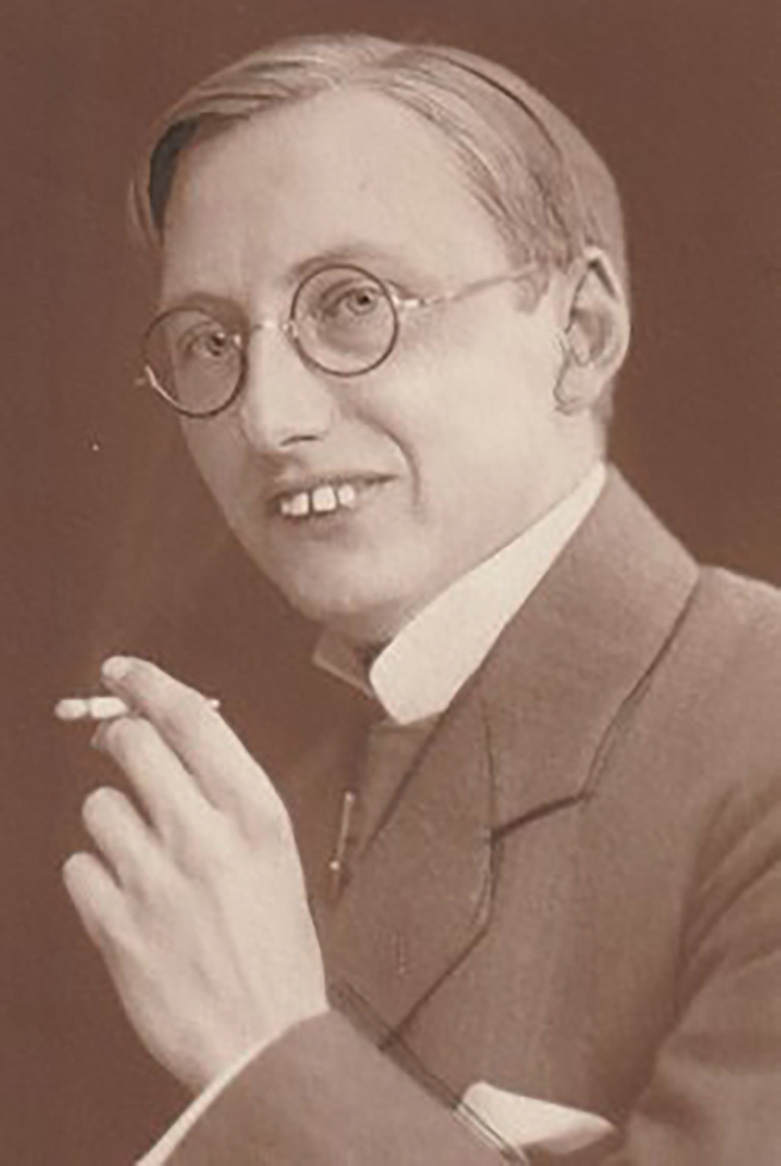
\includegraphics[width=.8\textwidth]{figures/Hjelmslev_young.jpg}
  \caption{Louis Trolle Hjelmslev as a young MA}
  \label{fig:ch.hjelmslev.young_hjelmslev}
\end{wrapfigure}
In 1917, {\Hjelmslev} entered Copenhagen University, where he studied
Romance and (later) comparative philology with a number of
distinguished figures, especially \name{Holger}{Pedersen}. Through {\Pedersen}'s
influence he became interested in \ili{Lithuanian}, and spent the year 1921
doing research in Lithuania, which resulted in his 1923 master's
degree for a thesis on \ili{Lithuanian} phonetics. The year after he
received his MA was spent in Prague, where his knowledge of
traditional \ili{Indo-European} studies was developed. This travel was
somewhat against his will: he had just been engaged to be married to
\name{Vibeke}{Mackeprang}, his future wife, and was very much in love.  He was
much happier to spend 1926 and 1927 in Paris, where he studied with
{\Meillet}, {\Vendryes}, and others; the attachment to things \ili{French} formed
at this time was a lasting one, as shown in the fact that during his
entire career the bulk of his writing in languages other than \ili{Danish}
was in \ili{French}.

In 1928 he produced a book (\citealt{hjelmslev28:principes},
\textsl{Principes de grammaire générale}) which aimed ambitiously at
providing a general theoretical foundation for the study of
language. The continuity between this book and his later work is
evident from its goal of developing an abstract formal ``system within
which the concrete categories are found as possibilities, each having
an exact location defined by the conditions for its realization and
its combination with other categories''
\citep{efj65:hjelmslev.obit}. This work was quite uncompromisingly
theoretical in nature: having read it, {\Pedersen} advised {\Hjelmslev} also
to produce something that would allow him to qualify for the doctorate
in his own field, \ili{Indo-European} Comparative Philology. he also
supported the publication of the \textsl{Principes} in the prestigious
series published by the Royal Academy, which also gave {\Hjelmslev} a
number of copies to send to other linguists he knew (about), a huge
advantage at the time.

{\Hjelmslev} thus used the \textsl{Principes} to make his views known as
a structuralist and theoretician, but also wrote \textsl{Études
  baltiques} \citep{hjelmslev32:thesis}, a rather traditional work of
historical phonology dealing with Baltic phonology and especially with
the principles governing suprasegmental factors in these languages:
\isi{tone}, \isi{accent}, and quantity. He defended this for the doctorate with
{\Pedersen}'s active help.  {\Pedersen}'s advice in 1928, 9 years before it
became relevant, had the effect of enabling {\Hjelmslev} to claim to be
qualified as a fully trained historical linguist when {\Pedersen}'s chair
became available (in 1937 when {\Pedersen} turned 70). Since the doctoral
degree had been granted by the University of Copenhagen with {\Pedersen}
on the committee, this was an impeccable qualification. Later 
\name{Viggo}{Brøndal} would try to prevent {\Hjelmslev} from being appointed to the
chair, precisely by pointing to his interest in general linguistics,
but {\Pedersen} could point to his doctoral degree as proof that he was a
qualified \ili{Indo-European} scholar (as well).

During the same period, he also undertook (by request) the editing of
the manuscripts and other writings of \name{Rasmus}{Rask}. He published three
volumes of {\Rask}'s manuscripts \citep{hjelmslev:rask} with commentary
and two volumes of letters in 1941. A final volume,
\citet{bjerrum68:rask}, consisting of a manuscript catalog and further
commentary, was published much later by his student \name{Marie}{Bjerrum}. 
{\Hjelmslev} was obviously fascinated by {\Rask} both personally
and intellectually: he considered that the general evaluation of this
scholar was completely misguided, and argued in
\citet{hjelmslev:rask.comentaire}, a paper given in Paris in 1950,
that the major goal of {\Rask}'s work, especially toward the end of his
rather short life, was not the development of historical linguistics
(the connection in which his name is generally cited), but the
development of a general \isi{typology} of linguistic structure in terms of
which a basically ahistorical comparison of languages would be
possible.

There is a certain amount of anachronism in the resulting picture of
{\Rask} as a pioneer of \isi{structuralism}, but probably less than is claimed
by \citet{diderichsen60:rask} in his attack on {\Hjelmslev}'s
interpretation. The central issue in this controversy has been whether
{\Rask} had a clear notion of the difference between typological and
genetic comparison as the basis for discussing linguistic
relationships. Though he probably did not, and thus should not be
credited with an explicit theory of synchronic linguistic structure,
his interest seems clearly to have been in the question of how
languages are to be compared with one another, and not simply in how
they evolve. Unfortunately, {\Rask} fits too conveniently into the
conventional wisdom about the development of comparative historical
linguistics in the nineteenth century, and (outside of a narrow circle
of specialists) {\Hjelmslev}'s view, based on a serious and extended
study of all of the available material, has not been seriously
integrated into standard histories of the field.

{\Hjelmslev}'s work in phonology can be said to date from 1931, the year
of the {International Congress of Linguists} in Geneva. At that meeting
the phonologists of the Prague school were actively proselytizing for
their novel approach to \isi{sound structure} (see
chapter~\ref{ch.prague}). One result of this was the formation of
`phonological committees' in various research centers; and {\Hjelmslev}
participated in the creation of such a committee in Copenhagen under
the auspices of the \isi{Linguistic Circle of Copenhagen} (founded on the
Prague model in 1931, on {\Hjelmslev}'s initiative: see
\citet{jensen.gregersen21:hjelmslev.jakobson} for a detailed account
of its aims and activities). The initial goal of this committee was
to produce a phonological description of \ili{Danish} according to Praguian
principles and as part of the \emph{Internationale Phonologische
  Arbeitsgemeinschaft,} as {\Hjelmslev} had promised {\Jakobson} when they
met at the {Second International Congress of Linguists} in
Geneva. Subsequently, however, {\Hjelmslev}'s work tended more toward the
creation of a general theory of \isi{sound structure} (and of language in
general), especially after he began to work together with \name{Hans Jørgen}{Uldall}.

{\Uldall}, born in 1907, had studied {English} in Copenhagen with {\Jespersen}
and, in 1927, in London with \name{Daniel}{Jones}. After teaching briefly in
Capetown (where he substituted for \name{D. M.}{Beach} at the remarkably young
age of twenty-two) and London, he went to the United States in 1930 to
do fieldwork on American Indian languages under {\Boas}. He spent
1931--32 in California working closely together with \name{Alfred}{Kroeber}.
He worked especially on Nisenan (``Southern Maidu''), and is said to
have become fluent in the language. He received his MA in Anthropology
from Columbia for this work under {\Boas}'s supervision in 1933 (though
he never submitted his thesis), and returned to Copenhagen (where he
had no real job awaiting him, a problem that was to plague him for
most of his professional life).

The collaboration between {\Hjelmslev} and {\Uldall} began shortly after his
return, within.the context of the `phonological committee'. Its first
concrete result was a paper \citep{hjelmslev.uldall35:phonematics} `On
the Principles of Phonematics', delivered to the Second International
Congress of Phonetic Sciences in London in 1935
(figure~\ref{fig:ch.firth.icphs_1935}) by {\Hjelmslev} and accompanied by
\posscitet{uldall36:london} presentation of the phonematics of
\ili{Danish}. While the picture of `phonematics' presented by {\Hjelmslev} is
close in spirit to Praguian `phonology, it also diverges quite clearly
in significant details. Importantly, {\Hjelmslev} and {\Uldall} reject both
the sort of psychological definition of phonemes (as the
`psychological equivalent of a \isi{speech sound}' or as the `intention'
underlying realized speech) characteristic of the very earliest Prague
school work under the influence of {\DeCourtenay}, and also any
sort of purely phonetic definition which would identify phonemes with
external physical properties of the speech event. Instead, they
require that phonemes be defined exclusively by criteria of
distribution, \isi{alternation}, etc., within the linguistic pattern, as
foreshadowed already in \posscitet{hjelmslev28:principes}
\textsl{Principes de grammaire generale}.

\begin{wrapfigure}[12]{r}{.5\textwidth}
  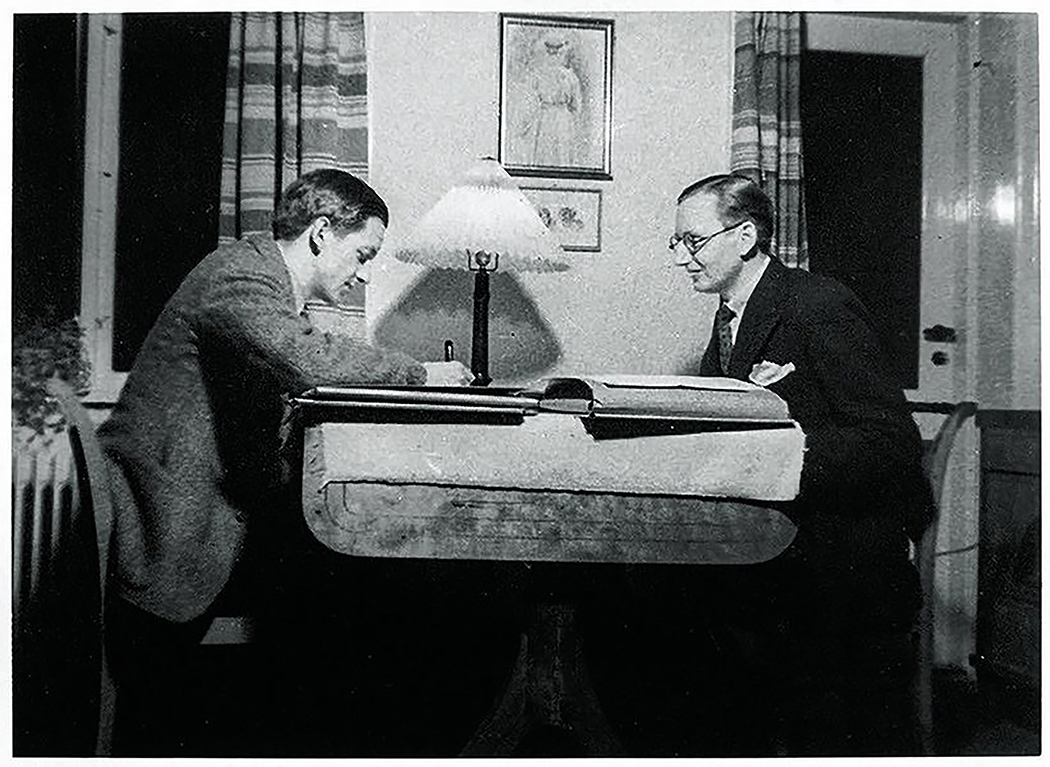
\includegraphics[width=.9\textwidth]{figures/Hjelmslev_and_uldall.jpg}
  \caption{Hans Jørgen Uldall and Louis Hjelmslev}
  \label{fig:ch.hjelmslev.uldall-hjelmslev}
\end{wrapfigure}
The differences between {\Hjelmslev}'s views and those of the Prague
phonologists were quite explicit; indeed, this is a point {\Hjelmslev}
insisted on many times. Virtually all of his papers dealing with sound
structure contain at least as an aside, and sometimes as the main
point, a reproof of `phonology' as making an important conceptual
mistake in basing its analysis on considerations of
substance—especially on phonetic properties. {\Hjelmslev}'s interaction
with both {\Trubetzkoy} and {\Jakobson} involved a considerable amount of
mutual criticism. This was never explicitly bitter or personal in tone
on either side, although \citet[17]{martinet85:hjelmslev} reports that
``[l]e refus de reconnaître toute dette envers Prague était, chez
{\Hjelmslev}, au moins partiellement déterminé par une hostilité
personnelle – le mot n'est pas trop fort – envers
Troubetzkoy''.\footnote{``The refusal to recognize any debts to Prague
  was, for {\Hjelmslev}, at least partially determined by a personal
  hostility – this word is not too strong – towards {\Trubetzkoy}''} The
feeling seems to have been mutual: after the presentation by
\citet{hjelmslev.uldall35:phonematics} at the Congress in London, in
which the basis of phonemic entities in phonetic substance was
strongly rejected in favor of purely formal criteria, {\Trubetzkoy} wrote
\citep[248]{liberman01:trubetzkoy.anthology} to {\Jakobson}, who had not
been present at the Congress, that ``To a certain extent, {\Hjelmslev} is
an enemy. [\ldots] I believe that {\Hjelmslev} is trying to ``out-Herod
Herod,'' that is, us.''  (See also
\citealt[22]{early.years:efj-rj.letters};
\citealt[19]{efj97:jakobson}).  As well as in his letter to {\Jakobson},
\citet[83]{trubetzkoy39:grundzuge} explicitly criticizes the point of
view of {\Hjelmslev}'s London paper.  Relations between glossematics and
other forms of structural linguistics seem never to have been
particularly warm either, although {\Jakobson} himself enjoyed warm
personal relations with {\Hjelmslev} over many years
\citep{efj97:jakobson}.

Since 1934, {\Hjelmslev} had been a reader in comparative linguistics in
Aarhus, where {\Uldall} had joined him in order to continue their joint
work. In 1937, {\Hjelmslev} succeeded {\Pedersen} in the chair of general
linguistics in Copenhagen (al\-though {\Uldall} was still without a regular
job). By this time, the two had decided that their views on
phonematics could be combined with {\Hjelmslev}'s earlier work on
grammatical categories (represented in his \textsl{Principes}, and also by his
work \citep{hjelmslev:case} on case, into a general theory of
language. Both felt that this was the first approach to language that
treated it in itself and for its own sake rather than as a combination
of the objects of other, non-linguistic disciplines—such as psychology,
physiological and acoustic phonetics, etc. A distinct name seemed
warranted to emphasize this difference from previous `linguistics',
and thus was born the field of \emph{glossematics}.

In order to give substance to glossematics, {\Hjelmslev} and {\Uldall}
wanted to provide a complete set of definitions and concepts that
would constitute a rigorous, internally consistent framework of
principles, founded on a bare minimum of terms from outside the
system. Such a theoretical apparatus would specify the sorts of formal
system that count as `languages' in the most general terms, and also
what constitutes an `analysis' of a language.

The latter notion is described in glossematic writings as a set of
`procedures' of analysis—probably an unfortunate term, since it
suggested the sort of field procedures a linguist not knowing a given
language might actually apply to arrive at an analysis of it. In
fact, the notion of `procedure' in glossematics is a specification of
the form a finished analysis takes, not the way one arrives at it. To
say that texts are made up of paragraphs, which are made up of
sentences, which are made up of clauses, etc., is to say nothing at
all about how to go about dividing up an actual text in practice, and
glossematics had no real practical hints to offer on this
score. Rather, it was assumed that the linguist went about learning
and analyzing a language using any methods or shortcuts that turned
out to be convenient: only after arriving at an analysis was it to be
organized so as to conform to the glossematic `procedure'.

{\Hjelmslev} and {\Uldall} kept developing and elaborating their analytic
framework and system of definitions, with the hopes of publishing soon
a detailed Outline of Glossematics. In 1936 at the International
Congress of Linguists in Copenhagen, they distributed a pamphlet of a
few pages \citep{hjelmslev.uldall36:outline}, identified as a sample
from a work of this title ``to be published in the autumn.'' No year was
specified for this ``autumn'' however, and it became a standing joke
among linguists in Copenhagen.\footnote{Such a long-delayed but
  much-referred-to work, supplying the conceptual underpinning for a
  good deal of other work, cannot fail to remind linguists of a more
  recent vintage of the \textsl{Sound Pattern of English}.}

In 1939, as the war was beginning, {\Uldall} finally was offered a more
secure position—in Greece, with the British Council. His departure
effectively severed the glossematic collaboration during the war
years, but the two continued to work independently on what they still
considered their joint project. {\Hjelmslev} completed a sort of outline
of the theory, but felt he ought not to publish it in {\Uldall}'s absence
(it was ultimately published as \citet{hjelmslev75:resume},
\textsl{Resume of a Theory of Language}). Instead, he produced
\citet{hjelmslev43:prolegomena}, a sort of introduction to the theory
and its conceptual basis, under the title \textsl{Omkring
  sprogteoriens grundlæggelse} (translated into {English} in 1953 with
some minor revisions as \citet{hjelmslev53:osg.whitfield},
\textsl{Prolegomena to a Theory of Language}, further revised in
collaboration with Whitfield\ia{Whitfield, Francis} as \citet{hjelmslev61:prolegomena}).

Though {\Hjelmslev} at least claimed to regard this as a sort of
`popular' work, indeed a work of ``vulgarization'', it is surely one of
the densest and least readable works ever produced in linguistics. It
is largely through this book (and reviews of it), however, that
linguists outside {\Hjelmslev}'s immediate circle came to know anything
about the substance of glossematics. In 1952, he taught in the
{Linguistic Society of America}'s Summer {Linguistic Institute}, where he
had an opportunity to present his views to a North American
audience. This event certainly made glossematics better known outside
Europe, but does not appear to have produced a great many converts to
the theory.

{\Hjelmslev} and {\Uldall} continued to work independently on the theory
over the following years, but were unable to spend much time
together. {\Uldall} was briefly in London, and held a succession of
positions in Argentina, Edinburgh, and later in Nigeria; he was able
to spend 1951-52 in Copenhagen, but by this time it appears that his
and {\Hjelmslev}'s views had come to diverge significantly. They still
hoped to bring out a unified Outline of Glossematics; in fact, {\Uldall}
published part 1 of such a work \citep{uldall57:outline}, but
{\Hjelmslev} found himself unable to write his proposed part 2 on the
basis of {\Uldall}'s presentation. {\Uldall} himself died of a heart attack
in 1957; and {\Hjelmslev}'s own time during the 1950s and early 1960s was
increasingly devoted to university administrative tasks rather than to
the further development of glossematics. Though he produced a number
of papers on particular topics, including at least one
\citep{hjelmslev54:stratification} with a general scope, he never
published any more comprehensive description of his theory beyond that
in the \textsl{Prolegomena}. He was very ill in his last years, and
died in 1965.

\section{Hjelmslev's notion of an `immanent' Linguistics}

Following {\Saussure}, {\Hjelmslev} regarded languages as a class of sign
systems: the essence of a language is to define a system of
correspondences between sound and sense. The analysis of a language,
then, involves describing each of these two \emph{planes} and their
interconnections. The domain of the Saussurian \emph{\isi{signifié}}—the
`meanings' of signs—{\Hjelmslev} calls the plane of \emph{content}, while
the domain of the \emph{\isi{signifiant}} is the plane of
\emph{expression}. Each of these planes in any given language has its
own structure: words (or morpheme-sized units, to reduce attention to
elements the size of a minimal sign) are realized by a sequence of
segments in the expression plane; and their meanings can be regarded
as combinations of smaller componential units in the plane of
content. Importantly, these two analyses of the sign are not
conformal, in the sense that units of expression are not related in a
one-to-one fashion to units of content. The word \emph{ram} /ræm/ in
\ili{English} can be regarded as a sequence of /r/ plus /æ/ plus /m/ in the
\isi{plane of expression}, and as the combination of \{male\} and
\{sheep\} in the \isi{plane of content}, but there is no exact one-to-one
correspondence between the two analyses.

{\Hjelmslev} considered that previous (and contemporary) linguistics had
failed to provide an analysis of either content or expression in terms
of its own, strictly linguistic or \emph{immanent} structure. In particular,
the linguistic analysis of content had been directed toward an account
of linguistic categories of \isi{meaning} based on general aspects of human
mental or psychological organization; while the analysis of expression
had attempted to reduce this aspect of linguistic structure to the
study of general \isi{acoustics} or physiological phonetics. In his opinion,
other linguists were attempting to study the categories of language as
special cases of more general domains, each of which (in particular,
psychology and phonetics) constituted a more comprehensive field that
was in principle independent of the special properties of language.

For {\Hjelmslev}, all such moves are fundamentally mistaken, in that they
obscure or deny the specifically \emph{linguistic} character of
language. The only way to study language in its own right, according
to him, was to develop a notion of linguistic structure completely
independent of the specifics of either phonetic realization or
concrete intentional meanings. The radicalism of {\Hjelmslev}'s project
lies in its seemingly paradoxical proposal to study systems of
correspondence between \isi{sound and meaning} with methods that are to be
completely independent of either sounds or meanings. His critics,
needless to say, did not fail to point out and even exaggerate the
apparent contradictions of such an approach.

I will discuss the basis and justifiability of this program below. At
this point it is worth pointing out, however, that in embracing it
{\Hjelmslev} became the first modern linguist to campaign specifically
against the notion that `\isi{naturalness}' in linguistics is to be achieved
by reducing facts of linguistic structure to facts from other, not
specifically linguistic, domains. This issue was often ignored in
later structuralist discussion; or misstated, as when {\Hjelmslev} is
cited simply as advocating the analysis of linguistic structure
without appeal to \isi{meaning}, ignoring the fact that phonetic facts are
in his terms just as irrelevant as semantic ones.

Indeed, in the strongly positivistic atmosphere of scientific studies
in the 1930s, 1940s and 1950s, it seemed hard to take seriously an
approach to language that renounced at the start a foundation in
operational, verifiable external facts. It would, in fact, be a
mistake to equate the kind of program against which {\Hjelmslev} was
actually reacting, one that saw the goal of linguistics as the
reduction of language to non-linguistic principles, with empiricist
approaches to the field in general. In advocating the complete
independence of linguistics from both semantics and (more importantly)
phonetics, however, {\Hjelmslev} left few substantive points of contact
between his view of glossematics and the empiricist linguistics of his
time—except for an appeal to rigor and explicitness, a kind of
`motherhood' issue that no scientist could possibly fail to
applaud. The fundamental presuppositions about the role of
`\isi{naturalness}' in linguistic structure against which {\Hjelmslev} aimed
his appeal for an immanent linguistics were not really discussed by
most of his critics. These concerns would reappear later, however, in
the context of post-\textsl{Sound Pattern of English} generative
phonology under conditions that make substantive discussion easier to
engage (see chapter~\ref{ch.spe} below, and
\citealt{sra81:unnatural}).

{\Hjelmslev} argues for the independence of linguistics from external
considerations (at least from the phonetic facts that might be thought
to play an essential role in the \isi{plane of expression}) by claiming that
in fact the same linguistic \emph{system} can be realized in radically
different media. In particular, the \isi{linguistic system} of a given
language can be realized either orally, in the sounds studied by
phoneticians, or orthographically, by symbols of an alphabet. Even
within the limits of phonetic realization, he suggests that arbitrary
replacements of one phonetic segment by another (so long as the same
number of contrasts remain, and the pattern of distribution,
\isi{alternation}, etc., of contrasting elements stays the same) would have
no effect on the system. If [t] and [m] were systematically
interchanged in all \ili{German} words, he suggests, the result would still
be identically the same system as that of standard \ili{German}.

Additionally, the same system could be realized in systems of manual
signs, flag signals, Morse code, etc.: a potentially limitless range
of ways to express what would remain in its essence the same
\isi{linguistic system}. If this is indeed the case, the system itself as we
find it can have no intrinsic connection with phonetic reality (to the
exclusion of other possible realizations). Reviewers and others
discussing glossematics replied that (a) orthographic and other
systems are obviously secondary in character, parasitic on the nature
of spoken language and developed only long after spoken language had
arisen; and (b) in any event, such systems do not in general display
the `same' system as spoken language.

To the first of these objections {\Hjelmslev} replied that the
historically second\-ary character of writing, etc., is irrelevant,
because what is important is the \emph{possibility} of realizing the
system in another medium, not the fact of whether this possibility was
or was not realized at some specific time. As to the supposedly
derivative character of writing, {\Hjelmslev} quite simply denied that
writing was invented as a way of representing (phonetically prior)
speech: he maintained that writing represented an independent analysis
of the expression system of language. If sound and writing both serve
as realizations of the same system of elements composing the
expression side of signs, it is only natural that they should show
close correspondences; but the lack of detailed isomorphism between
the concrete facts of \isi{phonetics} and \isi{orthography} in all known writing
systems, together with our obvious lack of knowledge of the specific
motivation and procedures of the inventors of writing, make the point
at least moot.

The content of the second objection noted above is that when one
studies the system of, for example, \ili{English} writing in \ili{Latin}
characters, one arrives at a rather different system than when one
studies \ili{English} phonetics. Written \ili{English} does not have contrastive
\isi{stress} (or any \isi{stress} at all, for that matter); it makes some
contrasts spoken \ili{English} does not (e.g., \emph{two} vs. \emph{too}
vs. \emph{to}), and \emph{vice versa} (e.g. \emph{read} [rijd]
vs. \emph{read} [rɛd]); the \isi{distinctive features} of the letters
involved (insofar as this notion can be carried over into such a
domain) establish rather different candidates for the status of
\isi{natural class} than do phonetic criteria; and so forth. Again, it could
be argued that this is beside the point: {\Hjelmslev} was quite ready to
concede that in practice rather different systems of expression form
(e.g., those corresponding to phonetic and to written norms) might be
matched to the same system of content form as variants of the `same'
language; but what matters is the fact that in principle it would be
\emph{possible} to develop a writing system that would mirror the same
system of expression as that operative in a given spoken
language. Indeed, an adequate system of \isi{phonemic transcription}
(perhaps representing phonemes as graphic feature complexes, somewhat
along the lines of the Korean Hangeul \isi{orthography}) would serve to make
{\Hjelmslev}'s point in principle.

Discussion of {\Hjelmslev}'s views in the literature, thus, cannot really
be said to have effectively refuted his position on the independence
of linguistic structure from external considerations. It would have
been to the point, perhaps, to question whether it is really accurate
to say that the character of the system would remain unchanged if
arbitrary substitutions were made in the realizations of its
elements. After all, the whole thrust of Neogrammarian \isi{explanation} had
been that the character of a synchronic state of language results from
the cumulative history of its accidental details. If such a state
represents a system, indeed, that fact must in some way grow out of a
combination of specific particulars; and those particulars must have
an influence on the development and maintenance of the system's
internal equilibrium. Though such an exclusively historical view of
language largely disappeared (outside of some Indo-Europeanist
circles, at least) with the rise of \isi{structuralism}, most linguists
would still agree that the working of \isi{sound change} and \isi{analogy} (both
crucially, though not exclusively, based in the details of the
external form of signs) contribute to the formation of the linguistic
system. If that is so, arbitrary changes in the external form of its
signs could not be said to leave the system of a language essentially
unchanged. The principal objections made to {\Hjelmslev}'s radical
position do not seem to have been based on grounds such as these,
however.

\section{Basic terms of glossematic analysis}

To make explicit the separation he intended between the system and its
manifestation, {\Hjelmslev} proposed a system of terms that has not
always been well understood by later writers:
\citet{efj66:form.and.substance,fischer-jorgensen75:trends} discusses
and clarifies this terminology and its history. First of all, he
proposed to distinguish between linguistic \emph{form} and linguistic
\emph{substance}: `form' is the array of purely abstract, relational
categories that make up the systems of expression and of content in a
given language, while `substance' is constituted by some specific
manifestation of these formal elements. Since the system itself is
independent of any concrete manifestation, and any such manifestation
only has a \emph{linguistic} reality insofar as there is a system
underlying it, {\Hjelmslev} maintained that ``substance presupposes form
but not vice versa.'' Although by the logic of the terms in question
this proposition is essentially tautologous, it was considered one of
his most controversial assertions. This is, of course, because it is
in this claim that the independence of linguistic structure from
phonetic (and semantic) reality becomes concrete.

A particular linguistic substance is regarded as the manifestation of
a given linguistic form in a particular \emph{purport}. This latter is
a kind of `raw material' subject to being used for linguistic
purposes, but which has no linguistic character in itself unless
shaped by a linguistic form into a linguistic substance. {\Hjelmslev}
uses the image of a net (representing form) casting shadows on a
surface (the \isi{purport}) and thereby dividing it into individual cells or
areas (the elements of substance). The complete range of human vocal
possibilities (considered as a multidimensional continuum) constitute
one sort of linguistic \isi{purport}, which can substantiate the
manifestation of a linguistic form (e.g,, the sound pattern of
\ili{English}) in a substance (roughly, the `phonemic' system of \ili{English} in
structuralist terms). In the nature of things, the same \isi{purport} may be
formed into different substance by different systems (e.g., the same
space of vocal possibilities is organized differently by different
languages), just as the same form may be `projected' onto different
\isi{purport} to yield different substances (as when both phonetic and
orthographic manifestations can serve to substantiate the system of
expression of the same language).

The notion of \isi{purport} is reasonably clear in the domain of expression
(given the ideas of `form' and `substance' in their glossematic
sense), but it is not so obvious that there is a range of potentially
different `purports' available to substantiate the content plane of
language, although the putative independence of language from
semantics implies that there ought to be.

The analysis of each plane, content as well as expression, involves a
search for the set of constitutive elements of signs within that plane
and for the principles governing the organization of these elements
into larger units. The specific glossematic implementation of this
search is the `\isi{commutation test}', according to which two elements of
linguistic substance in a given plane manifest different elements of
linguistic form if the substitution of one for the other leads to a
change in the other plane. In one direction, this is quite standard
structuralist procedure: phonemic \isi{contrast} exists between two phonetic
elements when substitution of one for the other leads to change of
\isi{meaning}.

An innovation in glossematics consists in the fact that the same
procedure is supposed to be applicable in looking for minimal elements
of content as well: thus, substitution of \{male\}+\{sheep\} for
\{female\}+\{sheep\} leads to a change in expression (from \emph{ewe}
to \emph{ram}), and so establishes \{male\} and \{female\} as
different elements of content form in \ili{English}. It must be added that
this program of analyzing content form as well as expression form by
essentially the same procedure remained a purely theoretical one, with
no substantial, extended descriptions of the glossematic content form
of particular languages ever having been produced. In general, the
complete symmetry of the two planes (expression and content) was a
major tenet of \isi{glossematic theory}; but in the absence of serious
studies of content form, it remained a point of principle with little
empirical content.

The `\isi{commutation test}' sounds like an eminently practical procedure;
indeed it resembles in its essentials the sort of thing students of
field linguistics in North America were being told to do in studying
unfamiliar languages. Seen in that light, however, it would seem to
compromise the claim that substance presupposes form but not vice
versa: if the only way form can be elucidated is by such a
manipulation of the elements of substance, its independence seems
rather limited. But here it is important to note that {\Hjelmslev} did
not at all mean the \isi{commutation test} to serve in this way: as observed
above, he felt linguists engaged in field description should make use
of whatever expedients helped them arrive at an analysis (including an
operational analog of the \isi{commutation test}, if that proved useful),
but that the validation of the analysis was completely \emph{ex post
  facto}, and not to be found in the procedures by which it was
arrived at. In other words, the analysis could perfectly well come to
the analyst fully formed in a dream: the role of the \isi{commutation test}
was to demonstrate its correctness as a formal system underlying a
particular association of content substance and expression substance.

The goal of linguistics, in glossematic terms, is the development of
an `algebra' (or \isi{notational system}) within which all possible
linguistic systems can be expressed. Such a theory specifies the range
of abstract possibilities for the systems of expression form and
content form in all languages, independent of particular
manifestations of such systems in specific substance. Each of the
`grammars' specified by such a theory is simply a network of
relationally defined formal elements: a set of categories available
for forming suitable \isi{purport} into substance.

The elements of such a network are themselves defined entirely by
their distinctness within the system (their commutability), and by
their possibilities of combination, distribution, \isi{alternation},
etc. The element of \ili{English} expression form which we identify with the
\isi{phoneme} /t/, thus, is not definitionally a voiceless dental stop but,
rather, something that is distinct from /p/, /d/, /n/, etc.; that
occurs initially, finally, after /s/, etc.; that alternates with /d/
(in the dental preterite ending), etc. The labels attached to such
minimal elements of expression form (and to corresponding elements of
content form) are completely arbitrary, as far as the system is
concerned: their identity resides entirely in their relations to other
elements, not in their own positive properties. Such a view is clearly
(and explicitly) an attempt to realize {\Saussure}'s notion of
\emph{langue} as form and not substance.

\begin{wrapfigure}{r}{.4\textwidth}
  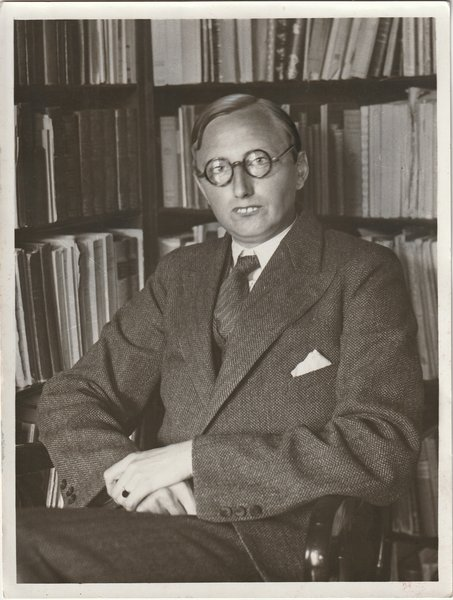
\includegraphics[width=.9\textwidth]{figures/hjelmslev_later.jpg}
  \caption{Louis Hjelmslev}
  \label{fig:ch.hjelmslev.hjelmslev2}
\end{wrapfigure}
As we have emphasized repeatedly above, it is this complete
independence between linguistic form and its manifestation in
substance that is both the hallmark and the most controversial aspect
of {\Hjelmslev}'s view of language. Taken in a maximally literal sense,
for instance, this separation seems to preclude any sort of even
halfway coherent analysis of actual languages: if we ignore
`substance', how are we to identify the initial and final variants of
a single phonetic type (e.g., [k])? Indeed, how can we even identify
initial [k] when followed by [i] with the [k] which is followed by
[u]? If we carry out a consistent analysis based on identifying
elements only by their possibility of commuting with others under
given distributional conditions, we arrive at an analysis in which,
for example, there are ten contrasting units initially before [i],
eight initially before [u], and six finally; but what basis do we have
for identifying the units found in one position with those found in
another, except their substantive (phonetic) resemblance? The issue is
reminiscent of the approach taken to the \isi{phoneme} by {\Twaddell}
(section~\ref{sec:twaddell} below).

For {\Hjelmslev}, the answer to this problem did not lie in conditions on
the possible form of grammars. In the general case, a variety of
different forms will be available for the same set of concrete
linguistic facts. The theoretical validity of any proposed formal
interpretation of a \isi{linguistic system} is assured by the fact that (a)
it satisfies the \isi{commutation test} (in that exactly those changes in
one plane that result in changes in the other are registered as
changes between distinct elements of the system), and (b) it satisfies
the oddly named `\isi{empirical principle}' in that the system itself is
internally consistent, exhaustive (i.e., accounts for all of the
facts), and as simple as possible (in that it posits a minimal number
of constituted elements in each plane). We will return to the
`\isi{empirical principle}' (and especially to the notion of \isi{simplicity} it
contains) below; for the moment, it is sufficient to note that this
principle considerably under-determines the formal interpretation of a
given linguistic usage.

The solution to the problem of providing a phonetically plausible
formal interpretation of a given usage lies rather in the way in which
a linguist matches a potential formal system (selected from the range
of possibilities given by the theory) to match that usage. The
linguist chooses that one of the formal possibilities which is most
appropriate to the substance, in that it provides the best and most
straightforward match between formal and substantive categories. Thus,
there is nothing in the nature of linguistic form that requires the
linguist to choose the `right' system (as long as the system he
chooses is one that satisfies the \isi{empirical principle}, and accounts
for commutation) — but there is nothing in the theory that prevents
him from doing so, either. The principles that govern the
appropriateness of particular formal interpretations of linguistic
usage fall outside of the study of form \emph{per se}, as they must if
substance is to presuppose form but not \emph{vice versa}.

This answer, while logically adequate, is unlikely to satisfy those
who feel {\Hjelmslev}'s separation of form from substance is too
radical. On the one hand, he is undoubtedly correct in insisting that
the system of language is centrally governed by properly
\emph{linguistic} principles, principles which cannot be reduced to
special cases of the laws of physiology, physics, general psychology,
logic, etc. But on the other hand, the categories of linguistic form
show too close a correspondence to those of substance to allow
linguists to treat this relationship as some sort of extra-systemic
consideration, or even as a colossal accident. By and large, the
\isi{regularities} of distribution, \isi{alternation}, and similar properties of
linguistic elements operate with reference to \emph{phonetically}
natural classes, have \emph{phonetic} explanations (at least in part),
etc.

Further, we see that linguistic systems when expressed in other media
than the phonetic show a similar dependence on, and determination by,
the properties of that medium. Striking demonstration of this has come
in the research on manual (or `sign') languages conducted since
roughly the 1960s. When {\Hjelmslev} wrote, the only such systems that
were generally considered by linguists were systems of finger
spelling, in which manual signs serve in a more or less direct way to
represent letters of an established \isi{orthography}—itself, in turn,
representing a spoken language.

With increasing attention to signed languages in their more general
form has come the realization that their structure falls within the
range of systems known from spoken languages, and that they are
grounded in the same cognitive and neural bases as spoken languages,
\emph{modulo} physical differences of modality. On the other hand,
they typically represent unique, autonomous systems that are quite
different in structure from (and not essentially parasitic on) the
spoken languages of the communities within which they are used. An
introduction to some basic properties of manual languages and their
distinctness from spoken languages is provided by
\citet{bellugi.klima79:sign}; a collection of results from the more
recent (massive) literature is provided by
\citet{brentari10:sign-languages}. While falling well within the class
of human natural languages, the organizing principles of these
systems, the natural classes of elements that function in linguistic
\isi{regularities} and the principles of \isi{historical change} operating on the
elements, etc., can only be understood in terms of the specific
characteristics of their manual implementation—suggesting that a
similar understanding of phonetic implementation is essential to an
account of spoken languages.

Paradoxically, language seems to be subject in its essence to its own
proper set of organizing principles, while its concrete details can be
largely related to extra-linguistic factors. This contradiction is
nowhere resolved (or even admitted) by {\Hjelmslev}, but his work has the
merit of stressing one side of the question so strongly as at least to
raise the issue. Many other investigators have asserted the autonomy
of linguistic structure, but few have been willing to follow this
proposition in its most absolute form nearly so far. Probably the only
view of phonology to pose the problem and a concrete solution to it is
that associated with {DeCourtenay} and {\Kruszewski} (cf. above,
chapter~\ref{ch.kazan}): here the extra-linguistic factors serve as
\isi{constraints} on the raw material that enters the \isi{linguistic system},
while the system itself is subject to its own distinct set of
principles. As we have already noted, this is more a program for
research than a concretely articulated theory, but it does propose an
account of what must be considered the most central issue raised by
{\Hjelmslev}: the relation between form and substance in linguistic
structure.

There are numerous other issues in general linguistics that are
addressed by {\Hjelmslev}'s work, but considerations of space preclude
further discussion here. On the basis of the overall account given
above of the conceptual foundation and goals of glossematics, I now
move on to the proposals made within that theory concerning sound
structure, and their instantiation in particular descriptions.

\section{Hjelmslev's approach to the description of sound structure}

The abstract character of the issues treated thus far in the present
chapter and their distance from actual empirical descriptions of
particular language data are completely typical of the writings for
which {\Hjelmslev} is known. His study of such theoretical topics was
not, however, carried out in as near total isolation from concrete
factual material as is sometimes believed. His early training in
{Indo-European} studies, for example, involved the study of a range of
languages necessary to pursue that kind of research. His work on
Baltic (especially \ili{Lithuanian}) for his doctorate involved direct
fieldwork, and forced him to pay attention to a set of descriptive
problems in the domain of \isi{accent} to which he would return numerous
times in his later, theoretical writings.

\begin{wrapfigure}{r}{.4\textwidth}
  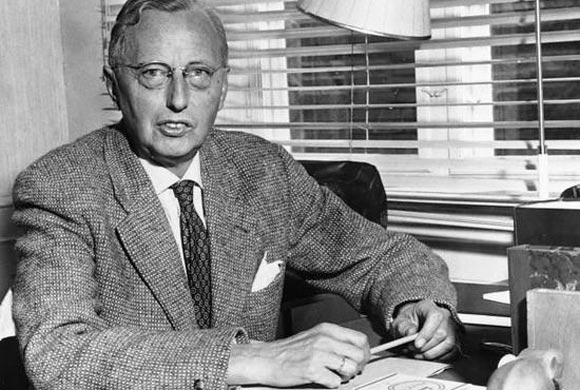
\includegraphics[width=.8\textwidth]{figures/Hjelmslev3.jpg}
  \caption{Louis Hjelmslev}
  \label{fig:ch.hjelmslev.hjelmslev3}
\end{wrapfigure}
In addition, he developed descriptive analyses of at least two other
languages in some detail: \ili{French} and \ili{Danish}. The description of \ili{French}
is known primarily from a summary by \name{Eli}{Fischer-Jørgensen} of lectures
{\Hjelmslev} gave in 1948-49 \citep{hjelmslev70:french}. The analysis of
\ili{Danish} is presented in an outline by {\Hjelmslev} himself
\citep{hjelmslev51:danish}, again representing lecture material rather
than a finished paper \emph{per se}. Despite its incompleteness and
inconsistencies, the analysis presented of \ili{Danish} is quite interesting
and substantial; it has remained little known because it appeared only
in \ili{Danish} in a comparatively obscure publication.  An {English}
translation has, however, been published as
\citealt[247--266]{hjelmslev73:essais.2}.

Of special help to present-day readers is the fact that {\Hjelmslev}'s
analysis of \ili{Danish} has been presented and extended by {\Basbøll} in a
series of two articles
(\citealt{basboll71:hjelmslev1,basboll72:hjelmslev2}; cf. also
\citealt{efj72:note}). {\Basbøll}'s aim is to demonstrate the potential
descriptive scope of a strictly glossematic analysis of sound
structure, and he stays explicitly within that framework in
explicating, improving, and further developing {\Hjelmslev}'s
analysis. According to \citet{efj72:note}, a number of {\Basbøll}'s
proposed modifications represent points that {\Hjelmslev} and others had
discussed informally and with which {\Hjelmslev} was more or less in
agreement.  More recently, \citet{basboll17:hjelmslev.french} provides
similar treatment of {\Hjelmslev}'s account of \ili{French}, and
\citet{basboll21:glossematics} updates and compares the two
glossematic analyses.

The sketchy analyses of \ili{Danish}, \ili{French}, and, to some extent,
\ili{Lithuanian} that we find in {\Hjelmslev}'s work perhaps raise more
questions about the descriptive methodology that should be attributed
to the theory of glossematics than they answer. Nonetheless, it is
possible to gain a reasonable idea of what such descriptions would
look like in practice from a study of the material referred to above,
especially that dealing with \ili{Danish}. The few other descriptions that
have been produced under the label of glossematics are not,
unfortunately, reliable as indicators of {\Hjelmslev}'s own views
\citep{fischer-jorgensen75:trends}. Within the scope of this chapter,
we cannot address all of the points of interest raised in {\Hjelmslev}'s
work. I attempt here only to give a notion of the dimensions along
which his views differed from those of his contemporaries, and
especially to present his views as they bear on the central issues of
this book.

For {\Hjelmslev}, the analysis of the expression system of a given
language starts from the set of elements that commute (or \isi{contrast})
with each other. These are all at least candidates for the status of
elementary constituents of the expression system; as we will see
below, however, the inventory may later be reduced if there are
reasons to represent some items as combinations or variants of others.

Within each of the two planes of language, the elementary constituents
of linguistic form are called \emph{taxemes}. These are the minimal
units that can be arrived at in any particular analysis: in the plane
of expression they are roughly the `size' of a segment (or
\isi{phoneme}). The point of introducing this terminology was (at least in
principle) to emphasize the independence of glossematic notions of
linguistic form, and especially its relation to substance, from their
`phonological' counterparts (primarily the views of the Prague school
and those of \name{Daniel}{Jones} --- see chapter~\ref{ch.firth}). The essential
difference is supposed to lie in the fact that \isi{taxemes} are elements of
pure linguistic form, having no necessary connection with
substance. The \isi{taxemes} could, of course, be manifested phonetically:
in that case, the units of phonetic substance that manifest them are
called \emph{phonematemes} by {\Hjelmslev}. These are roughly units
similar to structuralist phonemes, if we construe these as segments
given a `broad phonetic' characterization from which most or all
non-distinctive phonetic detail is omitted.

The \isi{taxemes} can be further dissolved into combinations of prime
factors called \emph{glossemes}. In scope, these units are comparable
(in the \isi{plane of expression}) to \isi{distinctive features}; but their
analysis is purely formal and universal, and depends in no way on the
actual phonetic content of the segments manifesting the
\isi{taxemes}.\footnote{At least in principle, although it is striking how
  much {\Hjelmslev} refers to phonetic substance in the end.} The
\isi{glossemes} in the \isi{plane of expression} are called \emph{cenemes} and
those in the \isi{plane of content} \emph{pleremes}. {\Hjelmslev} sometimes
refers more generally to elements as `cenematic' or `plerematic'
(i.e., as units of expression and content, respectively); and to
`cenematics' and `plerematics' as the study of expression and the
study of content. Since the analysis of \isi{taxemes} into \isi{glossemes} has
much less systematic significance for the questions of interest to us
here, I will ignore these terms below and treat \isi{taxemes} as the
minimal units of linguistic form in each of the two planes.

The \isi{taxemes} of expression form are themselves defined by the network
of relations into which they enter. In his
\citeyear{hjelmslev.uldall35:phonematics} (preglossematic) treatment,
{\Hjelmslev} divides the {rules} characterizing these into three classes:
(a) {rules} of grouping, which specify the distributional, clustering,
etc., properties of elements; (b) {rules} of \isi{alternation}, which specify
the replacement of one element by another under specified grammatical
conditions; and (c) {rules} of implication, which specify replacements
that take place under phonematic conditions. This last definition
cannot be taken literally, since phonematic realization is only one
possible manifestation of linguistic form (others being orthographic,
etc., as discussed in previous sections). The distinction being made
is nonetheless clear: alternations involve two or more distinct
expression-forms that correspond to the same content, where the choice
between them is determined by conditions only represented on the plane
of content; while implications involve conditions for the occurrence
of one or another form that are present in the expression plane
itself.

These three classes of {rules}, incidentally, are asserted by {\Hjelmslev}
to be mutually exclusive in governing the relation between particular
\isi{phonematemes}. This would entail, if correct, the claim that two
segments which alternate (under either grammatical or phonological
conditions) cannot be systematically related in cluster formation. He
illustrates this by arguing that in \ili{German} the voiced and voiceless
obstruents which alternate in syllable-final position do not co-occur
in clusters. No one has ever actually examined this claim in any
detail; if true, it would be a remarkable fact indeed about the sound
patterns of natural languages.

The notion that the units of a linguistic analysis are to be defined
in terms of their role in a network of {rules} is maintained in
{\Hjelmslev}'s later, more strictly glossematic work, though much heavier
emphasis there is put on {rules} governing distribution than on the
principles of \isi{alternation}. The basic idea is clearly related to (and
in part derived from) the same proposal by {\Sapir}, discussed below in
chapter~\ref{ch.sapir}.

Another influence on {\Hjelmslev} in this regard can be traced in his
papers on linguistic reconstruction, an enterprise in which he
believed that the purely relational character of \isi{taxemes} is strikingly
shown. The reconstruction of earlier, unattested stages of a language
(or family) proceeds in a way that is completely independent of any
actual claims about the pronunciation of that ancestral language, at
least in principle. The result is the establishment of a system of
pure relations, whose terms are correspondences among phonological
elements in related systems, but are not themselves phonetic
realities. In this connection, he invokes the notion of `\isi{phoneme}' as
used by {\Saussure} in his \textsl{Mémoire}: an element in the system of
a reconstructed language, as attested by a unique set of
correspondences in the daughter languages. As we have seen above
(chapter~\ref{ch.saussure_sound}), {\Saussure}'s later use of the term
\emph{phonème} in the sense of `\isi{speech sound}' was from {\Hjelmslev}'s
point of view diametrically opposed to this, but in fact {\Hjelmslev} had
read the \textsl{Mémoire} and been impressed with it long before he
devoted serious attention to {\Saussure}'s work in general linguistics.

While the distinctions among expression \isi{taxemes} are purely formal and
relational, they usually correspond to surface phonetic differences as
well. This is not always the case, however, since substance (here,
phonetics) does not alone indicate what is most important about an
element of the \isi{linguistic system}: its function, or role in the system
of relations. For instance, in his description of \ili{French}, {\Hjelmslev}
notes that \isi{schwa} must be kept phonologically apart from {[œ]}, not
because they differ in any phonetic way (they do not, at least in
`standard', conservative \ili{French}), but rather because \isi{schwa} can be
latent (deleted) or facultative (optionally inserted) under specified
conditions, while the presence of {[œ]} is constant in a given form. It
is precisely its behavior with respect to certain {rules} that
establishes \isi{schwa} as a distinct element of the system of \ili{French}
expression form.

Differences of this sort between formal and substantive categories in
language show up most clearly when we consider the role in {\Hjelmslev}'s
system of (a) \isi{neutralization} or \isi{syncretism}; and (b) reductions in the
inventory of \isi{taxemes} due to representing certain elements as
combinations or variants of others. I discuss these two aspects of
glossematic description below.

Neutralization is defined as the ``suspension of a commutation'' under
some specifiable conditions. The result of the fact that certain
(otherwise contrastive) elements fail to \isi{contrast} under the conditions
in question is an \emph{overlapping}; the element that occurs in this
position is called a \emph{syncretism}. For example, syllable-final
voiced and voiceless obstruents fail to \isi{contrast} in \ili{German}, and so the
final element of words like \emph{Bund} `association' and \emph{bunt}
`colorful' (both phonetically {[bʊnt]}) is the \isi{syncretism} `t/d'.

Clearly, a \isi{syncretism} in this sense is similar to an \isi{archiphoneme} in
the Prague school sense (cf. chapter~\ref{ch.prague}), but there are
also several differences between the two concepts. For one thing,
syncretisms are not limited (as archiphonemes are) to cases in which
the elements which fail to \isi{contrast} share certain properties to the
exclusion of all other phonological elements in the language. Such a
condition would make no sense in {\Hjelmslev}'s system, since \isi{syncretism}s
involve elements of linguistic form and not substance, and phonetic
features are aspects of substance. Also, \isi{syncretism}s are not limited
to the \isi{neutralization} of binary \isi{oppositions}, a condition on
archiphonemes imposed somewhat arbitrarily by {\Trubetzkoy}, as noted
above in chapter~\ref{ch.prague}.

Finally, and perhaps most importantly, \isi{syncretism}s are only posited
when there is an actual \isi{alternation} involved (as in the case of \ili{German}
\isi{final devoicing}), and not in cases where a particular \isi{contrast} simply
fails to appear in a given environment (as in the case of \ili{English}
\isi{stops} after {[s]}, where only phonetically voiceless, unaspirated
elements occur). The latter are treated simply as instances of
\isi{defective distribution} of certain phonological elements: it is a fact
about \ili{English} \isi{stops} that, while the voiceless ones appear after {[s]},
the voiced ones do not.

Although {\Hjelmslev} maintained that evidence from alternations was
necessary to the positing of a \isi{syncretism}, he did not in fact always
adhere to this in his practice. Thus, he posits an abstract consonant
`h' in \ili{French} (to account for the well-known class of \emph{h-aspiré}
words, which begin phonetically with a vowel but behave in liaison as
if they began with a consonant). This segment is uniformly syncretic
with ∅ (i.e., it is never realized phonetically), despite the fact
that there are no alternations to support the \isi{syncretism}.

On the other hand, once a \isi{syncretism} is established between certain
elements in a certain position, the same analysis is extended to other
forms which do not happen to show any \isi{alternation}. Thus, \ili{German}
\emph{ab} is said to end in the \isi{syncretism} `p/b' (not simply in `p')
even though it does not alternate, since other alternating forms
establish the syncretisms of voiced and voiceless obstruents in this
position.

This treatment leads to a difference between two conditions under
which a \isi{syncretism} may occur. In the case of alternating forms,
related words provide evidence of which element is basic to the
\isi{syncretism} (thus, \emph{Bunde} establishes that `d' underlies the
\isi{syncretism} `d/t' of \emph{Bund} `bund/t'); while no such evidence is
available for non-alternating forms (e.g., \emph{ab}). The \isi{syncretism}
in the latter case is said to be \emph{irresoluble}, as opposed to the
\emph{resoluble} \isi{syncretism} in `bund/t'. Naturally, the question of
whether a given \isi{syncretism} is resoluble or not is a property of
individual forms, not of syncretisms themselves, since a \isi{syncretism}
that was irresoluble everywhere would lack the sort of basis in actual
alternations necessary to establish it in the first place.

Syncretisms are divided into several sorts, though the difference is
primarily terminological. When the opposition between two elements is
suspended in favor of one of them (as when both voiced and voiceless
obstruents are represented syllable-finally in \ili{German} by voiceless
ones), the \isi{syncretism} is called an \emph{implication}. When the
representative of a \isi{syncretism} is distinct from either element (e.g.,
the \isi{neutralization} of various unstressed vowels in \ili{English} as \isi{schwa}),
it is called \emph{fusion}; the same term is applied to a \isi{syncretism}
represented by either of the neutralized elements, in free
\isi{variation}. An example of this latter situation is furnished by \ili{Danish},
where syllable-final `p' and `b' do not normally \isi{contrast}, but where
the \isi{syncretism} can be pronounced as either aspirated or not. A
special case of a \isi{syncretism} is a \emph{latency}: this is a \isi{syncretism}
between an overt taxeme and ∅. A \ili{French} form such as the adjective
\emph{petit}, for example, ends in a `latent' `t'. In fact, in
{\Hjelmslev}'s analysis, all final \isi{consonants} in \ili{French} are latent
(unless followed by a vowel, such as a \isi{schwa}—itself latent in final
position under most circumstances). That is, there is an implication
of a consonant to ∅ in this position.

Syncretisms form a part of the \isi{phonological system} of a language, and
a representation on the \isi{plane of expression} in which all \isi{syncretism}s
are indicated has a systematic status. When all possible \isi{syncretism}s
are resolved (including the supplying of latent elements, a process
called \emph{encatalysis}), we obtain another expression
representation which also has systematic status. Such a notation, in
which all possible resoluble \isi{syncretism}s are resolved, is called
\emph{ideal}, while the notation with \isi{syncretism}s indicated is called
\emph{actualized}. It is the \isi{actualized notation} that is directly manifested
in substance as a series of \isi{phonematemes}, but the \isi{ideal notation} that
serves as the basic expression form of a sign. Diagrammatically, the
relation among these elements of a description is as in
figure~\ref{fig:glossematic.description}.

\begin{figure}[ht]
  \centering
  \begin{tabular}{cccll}
    &\isi{ideal notation}&\rdelim\}{3}{1em}&&`bund'\\
    \isi{syncretism} {rules}&↓&&(Form)\\
    &\isi{actualized notation}&&&`bund/t'\\
    manifestation {rules}&↓\\
    &\isi{phonematemes}&\}&(Substance)&{[bʊnt]}
  \end{tabular}
  \caption{Components of a glossematic description: German \emph{Bund}}
  \label{fig:glossematic.description}
\end{figure}

{\Hjelmslev}'s \isi{ideal notation} for expression form is certainly rather
abstract. It clearly cannot be recovered uniquely from surface forms,
for example, which is a condition of great importance in most other
schools of structuralist phonology. His descriptions make clear that,
in practice, it is quite similar to \isi{representations} that in other
schools were called morphophonemic, or to the underlying
\isi{representations} of generative phonology. A number of important
differences separate {\Hjelmslev}'s picture of \isi{sound structure} from that
of generative phonology, however. One of these concerns the actualized
notation, which corresponds to nothing in a generative description,
but which is assigned systematic significance in glossematics. On the
other hand, the multiple (unsystematic) intermediate \isi{representations}
in a classical generative or morphophonemic description have no
correspondents in {\Hjelmslev}'s picture, since his {rules} all apply
simultaneously rather than in an ordered sequence.

Another difference lies in the fact that no syntactic or other
grammatical information is in principle allowed in ideal
notations—leading, as
\citet{basboll71:hjelmslev1,basboll72:hjelmslev2} observes, to rather labored
analyses in cases where different word classes show systematically
different phonological behavior. This constraint follows, of course,
from the fact that such information concerns content, while ideal
\isi{representations} are an aspect of linguistic expression, and the two
planes are quite distinct in {\Hjelmslev}'s view. As a result,
grammatically conditioned alternations are represented as the relation
of two systematically different expressions that correspond to the
same content, while phonologically conditioned \isi{variation} is
represented as a relation between a single ideal expression form and
its various actualized correspondents.

\section{The role of simplicity in a glossematic description}

The distance between {\Hjelmslev}'s `cenematic' \isi{representations} and
phonetic ones is further increased by the fact that he makes every
possible effort to reduce the taxeme inventory by treating some
elements as variants or combinations of others. To this end, he makes
extensive use of aspects of \isi{representations} that others might consider
arbitrary.

An important role in this respect is played by the notion of
`\isi{syllable}' (cf.  section~\ref{sec:nonseg-struct}). Since {\Hjelmslev}
explicitly denied that any phonetic definition of syllables was
relevant to their identification and delimitation, he was largely free
to posit them wherever they seemed useful. For example, he noted that,
in \ili{German}, only {[z]} and not {[s]} occurs in undoubted
syllable-initial position (e.g., when word-initial); while {[s]}
occurs to the exclusion of {[z]} in undoubted word-final
position. Medially, the two \isi{contrast} in, e.g., \emph{reisen} `to
travel' (with {[z]}) \emph{vs}. \emph{reißen} `to tear' (with {[s]});
but here {\Hjelmslev} proposes to treat the \isi{contrast} as a matter of the
location of \isi{syllable} \isi{boundaries}—`rai.sən' vs. `rais.ən'. In this way
the two segments are reduced to positional variants of a single
one. Similarly, the small number of superficially contrastive
instances of the `ich-Laut' [ç] in \ili{German} (in e.g. \emph{Kuhchen}
`little cow', as opposed to \emph{kuchen} `to cook', with {[x]}) are
treated as differing in syllabic position (`ku.xən' vs. `kux.ən'),
removing the need to posit a rather counterintuitive phonological
difference between palatal and velar \isi{fricatives} (see
chapter~\ref{ch.structuralists} below for the attempt to represent
this difference within American structuralist theory as depending on
another sort of inaudible boundary element).

Similarly, a single segment may be represented as the manifestation of
a cluster. In \ili{Danish} (and other languages), {[ŋ]} can be represented
as manifesting `n' before `k' or `g', where `g' is itself often latent
in this situation. Thus, apparently distinctive {[ŋ]} can be treated
as the only overt manifestation of the cluster `ng'.  In this
instance, the single segment does not actually manifest a cluster \emph{per
se}; but the difference between {[n]} and {[ŋ]} is the difference
between simple `n' and `n' forming a cluster with a latent `g'.

Somewhat different formally is {\Hjelmslev}'s proposed reduction of
aspirated \isi{stops} {[p]}, {[t]}, and {[k]} in \ili{Danish} to clusters of `b',
`d', and `g' with `h'. In fact in initial position, the \isi{stops}
\emph{p}, \emph{t} and \emph{k} in \ili{Danish} are aspirated, and thus an
analysis of `p' as `bh', etc., would be phonetically realistic; but
there are two objections to this. First, the phonetic fact is entirely
a matter of substance, and as such strictly irrelevant to the analysis
of form. More importantly, though, {\Hjelmslev} in fact writes `hb',
`hd', and `hg' in most cases rather than `bh', etc., and there is no
phonetic justification whatever for this. Ultimately, he resolves this
issue by an appeal to distributional \isi{regularities}, as will be
described below.

Apart from the choice of `hb' over `bh' for `p', however, this
analysis raises a classic problem which is as real for any other
theory as for {\Hjelmslev}'s: how far should an analysis go in reducing
surface diversity to a small number of basic elements? In its most
extreme form, such reduction would allow every language to be reduced
to a system of one or two underlying elements, such as the `dot' and
`dash' of the Morse code. {\Hjelmslev} explicitly renounces any such
reduction, saying reductions should only be made when they are not
`arbitrary'; but the problem is precisely to provide a suitable notion
of `arbitrary' to constrain analyses. Intuitively, the reduction of
{[ŋ]} to `ng' is less arbitrary than that of {[p]} to `hb', but
(especially in the absence of considerations of substance) it is hard
to make this intuition precise. It cannot be said that {\Hjelmslev}
provided any explicit criterion for when a proposed reduction is
allowed, and when it is disallowed as `arbitrary'.

One might argue that, in fact, the principle {\Hjelmslev} appeals to in
distinguishing \isi{syncretism}s from \isi{defective distribution} is of relevance
here: that {rules} have to be founded in alternations (in the most
general sense of the term) in order to be justified. This condition
would allow the representation of \isi{nasal vowels} in \ili{French} as ideal
sequences of vowel plus \isi{nasal consonant}, for example, as argued by
{\Hjelmslev}, and perhaps the representation of \ili{Danish} {[ŋ]} as `ng'. It
would, however, prohibit the representation of \ili{Danish} \emph{p},
\emph{t} and \emph{k} as combinations of `b', `d' and `g' preceded by
`h' (though {\Hjelmslev} does attempt to adduce evidence from
alternations in loanwords such as \emph{lak} {[lagͦ]} `lacquer (n.)'
\emph{vs}. \emph{lakere} {[lagͦhe':rə]} `to lacquer (vb.)'). More
drastically, it would prevent any sort of analysis in which two
segments that are in \isi{complementary distribution} (but do not alternate)
are represented as the same underlying element: for instance,
{\Hjelmslev}'s treatment of \ili{Danish} \isi{syllable} initial {[t]} and final {[d]}
as representing the expression taxeme `t', while initial {[d]} and
final {[ð]} represent `d'; or his elimination of the vowel {[œ]} from
the \ili{Danish} vowel system, as a variant of `ø'.

In fact, while the requirement of an \isi{alternation} to support a rule
makes obvious sense in the case of \isi{syncretism}s, it is not clear how
such a condition could be coherently formulated with reference to
{rules} of manifestation—and most of the problematic cases of possibly
spurious reductions fall within this area. {\Hjelmslev} does indeed argue
for the plausibility of certain reductions to manifestation {rules} by
invoking productive {rules}. For example, in discussing quantity in
\ili{Lithuanian}, he notes that there are certain semi-productive
alternations between long and short vowels; and then observes that the
same \isi{alternation}, in terms of its grammatical conditioning, relates
the vowels \emph{a} and \emph{o}, and \emph{e} and \emph{ė} (with the
first of each of these pairs occurring in the categories that show
short vowels, and the second in categories that show long vowels). On
the basis of this rule, he concludes that \emph{o} and \emph{ė} should
be treated as the long correspondents of \emph{a} and \emph{e},
respectively. Since his analysis treats long vowels as clusters of
short vowels, this allows him to eliminate \emph{o} and \emph{ė} completely
from the inventory of \ili{Lithuanian} expression \isi{taxemes} (treating them as
`a͡a' and `e͡e', respectively). It is by no means clear, however, that
similar arguments can be provided for all cases in which some segment
is eliminated from the inventory by treating it as a manifestation of
another.

For {\Hjelmslev}, the overriding condition motivating the reduction of
taxeme inventories is that portion of the `\isi{empirical principle}'
referred to above that requires a description to be as simple as
possible. In fact, the \isi{meaning} of `\isi{simplicity}' here is quite clear and
explicit: the simplest description is the one that posits the minimum
number of elements. On this basis, subject to the essential but
unclarified prohibition of `arbitrary' analyses, the linguist must
obviously make every reduction possible.

Interestingly enough, the notion of minimizing the number of elements
posit\-ed in an analysis has two quite distinct senses for {\Hjelmslev},
with rather different implications. On the one hand, of course, it
refers to minimizing the taxeme inventory: it is in this way that the
reduction of \ili{Danish} {[p]} to `hb' is motivated by the principle of
\isi{simplicity}. In addition, however, the principle is used to motivate
the positing of \isi{syncretism}s.

This is because an analysis which assigns two different expression
forms to the same content form (i.e., which treats an \isi{alternation} as
grammatically conditioned or suppletive) is taken to posit more
`elements' (here, in the sense of sign expressions) than an analysis
which assigns a single, constant expression form to a single content
form. Thus, the principle that morphological elements should be given
unitary underlying forms wherever possible (often taken to be a
hallmark of generative phonology, and of morphophonemic analysis) is a
governing one in glossematic analyses. Of course, not all differences
in the expression of a single element of content can be so treated, as
{\Hjelmslev} recognizes: \ili{English} \emph{be}, \emph{am}, \emph{are}, etc.,
cannot be described by {rules} of \isi{syncretism} in the plane of
expression. A considerable range of (often, rather idiosyncratic)
alternations \emph{are} so treated, however: in his analysis of
\ili{French}, {\Hjelmslev} proposes a specific rule that makes the sequences
`sə', `fə' latent before `z' to account for the small number of
unusual words like \emph{os} ({[ɔs]} `bone', pl. {[o]} with the ideal
notation `osəz') and \emph{bœuf} {[bœf]} `ox', pl. {[bø]} with the
\isi{ideal notation} `bœfəz').

It is essential to recognize that the notion of \isi{simplicity} invoked by
{\Hjelmslev} is only applicable to inventories, whether of \isi{taxemes} or
sign expressions, and not at all to the {rules} or other statements of
\isi{systematic relations} that enter into the analysis. This is at first
sight somewhat at variance with his overall theoretical premises:
after all, the units (\isi{taxemes}, etc.) of the analysis only have their
existence insofar as they are defined by the network of \isi{rules} and
relations into which they enter; so it would seem reasonable to claim
that the primary way in which an analysis is `simple' is in having
simple {rules}. Nonetheless, it is clear that \isi{simplicity} of {rules} plays
little systematic role in {\Hjelmslev}'s thinking. For example, the
elimination of {[œ]} from the expression taxeme inventory of \ili{Danish} is
a comparatively limited gain in comparison with the complexity of the
{rules} which are necessary to predict it as a variant of `ø', but this
consideration is never raised in relation to the analysis, and it
would appear that it was quite irrelevant to the decision to make the
reduction in question.

Given that the elements of the analysis are supposed to derive their
reality only from the {rules} that relate them, a condition such as that
part of the \isi{empirical principle} which requires their number to be
minimized seems quite unfounded; but we must recognize that {\Hjelmslev}
probably approached the issue from a rather different vantage
point. After all, previous linguistics (including the earlier forms of
\isi{structuralism} with which he was familiar) had discussed sound
structure in terms of a theory of \emph{phonemes}, elements which
represented in one way or another the minimal contrastive constituents
of sound patterns. {\Hjelmslev} argued that these minimal elements of
form should be derived in a purely immanent way from the relations
among them, and to that extent emphasized the role of the {rules} in
grounding an analysis; but he does not seem to have escaped in his own
thought from the tendency to hypostatize the terms of these
relations. Though his is clearly a theory that differs from others in
the ontological status assigned to `phonemes', it is still primarily a
theory of units rather than a theory of relations in its actual
content and application. As such, the notion that \isi{simplicity} of
relations (and not simply of inventories) should play a role in the
theory does not seem to have occurred to him.

To the claim that \isi{simplicity} of {rules} played no part in {\Hjelmslev}'s
notion of phonological theory, two partial exceptions come to mind—one
more significant than the other. On the one hand, he maintained
consistently that the following constraint applied to consonant
clusters in all (or at least nearly all) languages: if
C$_{1}$C$_{2}$C$_{3}$ is a possible cluster, then both C$_{1}$C$_{2}$
and C$_{2}$C$_{3}$ must be possible as well. In other words, all
clusters of more than two elements must be made up of sequences that
are well formed in a local, pairwise fashion as well. It is this
constraint, in fact, that causes him to represent \ili{Danish} {[p]} as `hb'
rather than `bh' in many cases: if a cluster such as {[pl]} were
represented as `bhl', this would violate the condition because `hl' is
not otherwise possible in \ili{Danish}.

The relevance of this constraint to the \isi{simplicity} issue comes from
the fact that it might be seen as a requirement that the {rules} of
consonant clustering be `simple' in the particular sense that the
{rules} for long clusters be reducible to the {rules} for shorter
ones. The notion that this is a question of \isi{simplicity} of {rules},
however, does not seem very plausible. {\Hjelmslev} fairly clearly
regarded this generalization about clusters as having the status of an
independent principle of linguistic structure, and not at all as a
theorem to be derived from the requirement of \isi{simplicity} applied to
the {rules} of an analysis.

Another fact is perhaps more significant. Recall that, as stated
above, a large number of formal analyses are typically provided by the
theory of glossematics for any particular language, where the choice
among them is to be made on the basis of which analysis is most
appropriate to the substance in which the language is realized. This
cannot be interpreted otherwise than as the requirement that the {rules}
of manifestation be maximally simple. Of course, since the {rules} of
manifestation are not an aspect of linguistic form at all \emph{per
  se}, it is clear that the requirement of \isi{simplicity} in the empirical
principle (a principle that governs the range of possible linguistic
forms) cannot be responsible for this; but it is nonetheless a
consideration which would have a role to play in a more fully
elaborated \isi{glossematic theory} of \isi{sound structure}.

Simplicity of {rules}, then, may play a role in the relation between
linguistic form and its manifestation, but apparently not in the {rules}
underlying linguistic form itself. From this, and the expulsion of all
phonetic (or `substance') considerations from the analysis of form, it
might seem that the theory is hopelessly unable to deal adequately
with the nature of linguistic structure. One could maintain, for
example, that no analysis of \ili{German} can be said to describe the sound
pattern of the language unless it treats the changes of /b/ to /p/,
/d/ to /t/, etc. in \isi{syllable} final position as aspects of a unitary
fact; and it is only the requirement of \isi{simplicity} of {rules}, combined
with the definition of the segments involved as a substantive natural
class, that has this consequence.

To this objection, {\Hjelmslev} would probably have replied that it
states the issue backwards. In his terms, that is, it is the fact that
/b/, /d/, /g/, etc. undergo syllable-\isi{final devoicing} that establishes
the link among them, not their phonetic similarity. Different
languages containing the same segments may assign them quite different
phonological properties (a point made most explicitly by {\Sapir};
cf. chapter~\ref{ch.sapir} below), and so phonetic properties cannot
be taken as diagnostic in themselves of whether or not a class of
segments is phonologically `natural'. The very fact that the
implications affecting all of the voiced obstruents in \ili{German} have the
same form is what constitutes the similarity among the segments
involved—not the substance property of voiced implementation.

Of course, to make this notion more explicit it is still necessary to
develop a notion of when a set of implications (or other {rules}) are
relevantly `similar' to one another; but it is clear that such a
notion of rule similarity, implicit in glossematic notions, could be
formulated in a purely immanent way—that is, based on the form of
{rules} rather than on the substantial content of either {rules} or
segments. In fact, it was just such a principle of formally based rule
collapsing that underlay the notion of \isi{simplicity} characteristic of
early work in generative phonology (chapter~\ref{ch.spe}). In this
theory it was in effect proposed that the only intrusion of substance
into this question was through a universal phonetically based notation
system (the set of \isi{distinctive features}) for linguistic forms. A
perceived failure of this theory due directly to its attempt to
disregard the substance of {rules} (as opposed to \isi{representations}) was
responsible for the addition of the notion of `\isi{markedness}' in the
final chapter of \citet{spe}.

These issues take us increasingly away from the theory of
glossematics, at least as far as it exists in {\Hjelmslev}'s writings and
analyses. It is worth noting, however, that that theory raises rather
directly a number of questions that are less evident in relation to
other forms of \isi{structuralism}, and that would only be treated
systematically in much later work.

\section{Nonsegmental structure in glossematic phonology}
\label{sec:nonseg-struct}

Another aspect of {\Hjelmslev}'s theory which distinguishes it from most
of its contemporaries, and which has considerable relevance to
present-day work is the attention he paid to phonological structure
and properties that cannot be localized within the scope of a single
segment. Of course, other theories of phonology recognized the
existence of a certain range of `suprasegmental' properties, and in
fact the major contribution of the British school of \isi{prosodic analysis}
(chapter~\ref{ch.firth}) was precisely in this area. Nonetheless,
{\Hjelmslev} is unique among structuralists in the importance he accorded
to questions of \isi{syllable} structure and prosodic phenomena within a
primarily segmental framework.

\begin{wrapfigure}{l}{.35\textwidth}
  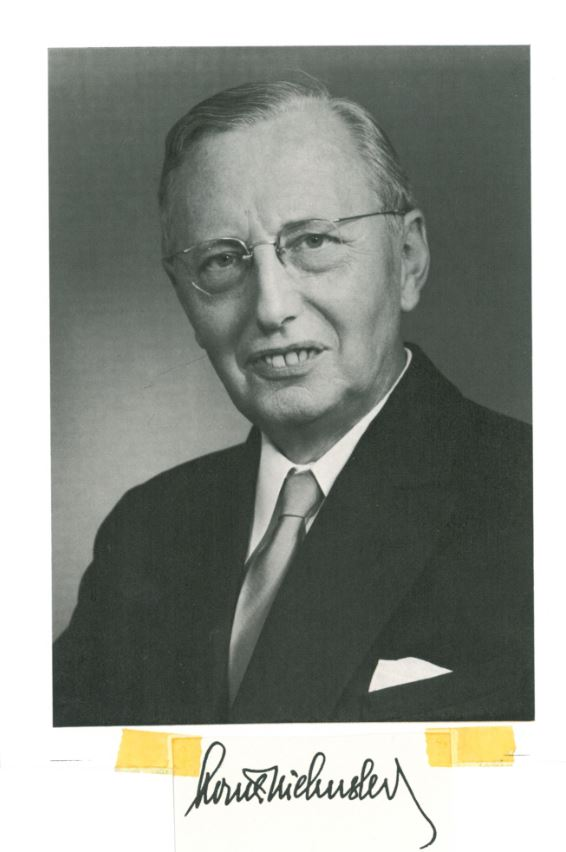
\includegraphics[width=.9\textwidth]{figures/Hjelmslev.jpg}
  \caption{Louis Hjelmslev}
  \label{fig:ch.hjelmslev.hjelmslev}
\end{wrapfigure}
Centrally, {\Hjelmslev} regarded a text as organized in a hierarchical fashion: into
paragraphs each of which can be divided into sentences, which can in
turn be divided into clauses that are divisible into phrases, etc. Of
particular interest for phonological analysis, a phrase (which can
represent a complete utterance by itself) is divided into syllables,
and each \isi{syllable} is divided into segments. Syllables thus play an
important role in organizing the utterance: they are the building
blocks of phrases, and the domains within which the distribution of
segments is to be specified.

It might be possible to give a phonetic definition of the \isi{syllable},
but (as noted above), this would be irrelevant to the analysis of
linguistic form even if such a substance-based characterization were
available. What matters to the analysis of linguistic form is a
functional definition of the \isi{syllable}, and {\Hjelmslev} proposes several
at various stages in his writings. The one he finally settles on,
which appears prominently in his descriptive work, is the following: a
\isi{syllable} is the hierarchical unit of organization that bears one and
only one \isi{accent}.

To understand this, we must of course ask how an `\isi{accent}' is to be
defined. The answer rests on {\Hjelmslev}'s view of the nature of
phonologically relevant properties. In the course of an analysis
(i.e., a division of a text into successively smaller hierarchical
units), one eventually arrives at units that cannot be further
subdivided (essentially, at the division of the utterance into
segments). These units can be said to constitute the chain that is a
text. But in addition to these, other relevant properties appear in
the text which are not localized uniquely in a single such
unit. Examples of such properties are intonations (which occur over an
entire utterance), \isi{stress} (which occurs over an entire phonetic
\isi{syllable}), \isi{pitch} accents in languages like \ili{Lithuanian}, which occur
over a sequence of vowel(s) and following sonorants, etc. Another
example is the \emph{stød} in \ili{Danish}: though this is realized in its
strongest form \citep{gronnum.basboll01:stod,gronnum.etal13:stod} as a
quasi-segmental element (a glottal stop, with associated perturbation
of laryngeal activity), {\Hjelmslev} analyzes it as a signal for certain
types of \isi{syllable} structure. The stød is a property of certain
segmental patterns within a larger hierarchical unit, rather than a
segment \emph{per se}.

Such an element that ``characterizes the chain without constituting
it'' is called a \emph{prosodeme}: these are in turn divided into two
types: \emph{modulations}, which characterize an entire utterance as
their minimal domain (e.g., intonation patterns that characterize
questions), and \emph{accents}, which do not (e.g., \isi{stress}, \isi{pitch}
\isi{accent}, the stød, etc.). It is in terms of this notion that {\Hjelmslev}
defines the \isi{syllable} as a hierarchical unit bearing one and only one
\isi{accent}.

Interestingly, since (on his analysis) none of these elements are
present in \ili{French}, he concludes that in the absence of accents, \ili{French}
has no syllables \citep{hjelmslev39:syllable}. Such a conclusion is
typical of {\Hjelmslev}'s intellectual style: he liked very much to use
the consequences of a rigorous set of definitions to derive striking,
indeed shocking conclusions.

This theory bears some resemblances to the proposals of
Metrical Phonology, at least in outline
(chapter~\ref{ch.otlabphon}). Both depend essentially on the notion
that utterances are organized into hierarchical units, and both claim
that certain properties are associated with units at one level while
others are associated with units at another level. The view of \isi{stress}
as a property of syllables, for example, can be opposed to
\posscitet{spe} view of \isi{stress}, which treats it as a property of
individual vowels (just as, e.g., height, backness, or rounding is a
property of a vowel). As opposed to Metrical Phonology, {\Hjelmslev}
appears to treat \isi{stress} not as a relation between syllables but as a
property (typically `strong \isi{stress}' vs. `weak \isi{stress}') which is
assigned to a particular \isi{syllable}. Since `weak \isi{stress}' presupposes
`strong \isi{stress}', though, and this relation might appear at several
\isi{levels}, it may well be that apparent differences between {\Hjelmslev}'s
view of the nature of \isi{stress} and that characteristic of Metrical
Phonology are merely a matter of notation.

An interesting aspect of {\Hjelmslev}'s theory of \isi{syllable} structure is
that he uses it to define the notions of vowel and consonant. A vowel
is defined as a segment that can constitute a \isi{syllable} by itself, or
as one that has the same distribution as such a segment. Consonants
are segments that do not fall into this category and that can appear
in various positions dependent on vowels.\footnote{For \ili{French}, which
  as noted above his account mandates the absence of syllables,
  {\Hjelmslev} establishes a category of ``pseudo-vowels'' on the basis
  of words consisting of only a single segment (\emph{à, ai, y, eau,
    ou, eu}) in order to make the relevant distinctions
  \citep[217]{hjelmslev70:french}.}  The definitions offered are not
always as precise and adequate as one might wish, but the view of
syllabicity that is involved is fairly clear. Syllables, that is,
contain an obligatory \isi{nucleus} and various optional peripheral
positions (which depend on the particular language). A segment
occupying the position of the \isi{nucleus} is \emph{ipso facto} a vowel
(regardless, as {\Hjelmslev} points out, of its articulatory properties:
liquids, nasals, and even some obstruents can be `vowels' if they
occupy the appropriate position in the \isi{syllable}), while a segment
whose dependence on such a \isi{nucleus} has to be specified within the
\isi{syllable} (i.e., part of an onset or syllable-final margin) is
\emph{ipso facto} a consonant.

The \isi{syllable} as a hierarchical unit thus has properties (e.g.,
accents) associated directly with it, rather than with its constituent
segments; it also has an internal structure which is essential to
defining the traditional notions of vowel and consonant. As a
hierarchical unit of linguistic form, it must of course first be
identified in terms of some relational properties it exhibits, and the
basis of the unit in these terms is its role in the statement of
segmental distributions. For {\Hjelmslev}, this was an extremely
important fact: the \isi{syllable} is the domain within which the grouping
properties of segments are defined, and (aside from special
restrictions that refer to \isi{boundaries} of the larger unit, the
utterance) this is the only such unit.

He explicitly denies, for example, that there are any grouping
restrictions that apply precisely to units of the size of a morpheme,
insofar as this is not coextensive with a \isi{syllable}. This impossibility
is claimed to follow from the separation of the planes of expression
and content: morphemes, as content units, have no autonomous existence
on the expression plane. Any limitations on the distribution of
expression units must thus be stated in terms of properties of the
expression plane, and it is exactly there that syllables have their
reality. Actually, since {\Hjelmslev} appears to count sign expressions
as units whose inventory should be minimized, it is not clear that
this consequence follows; but it is clear that {\Hjelmslev} intended the
\isi{syllable} to have this central role as the locus of distributional
restrictions.

One other such strange conclusion results from the definition of a
`consonant' . A segment only qualifies for this status insofar as its
distribution within the \isi{syllable} has to be specified; thus, a
hypothetical language with exclusively (C)V syllables, in which the
distribution of any consonant is completely determined by the fact of
its belonging to a specific \isi{syllable}, would have no `\isi{consonants}'. The
consonantal segments, that is, could be treated as a sort of prosodic
property of their syllables. In fact, he describes the earliest
reconstructable stage of \ili{Indo-European} as having this property: all
syllables were open, and instead of having `\isi{consonants}' in the strict
sense, the language had a large inventory of `converted
prosodemes'. This is claimed to be an unstable situation, which led to
radical restructuring of the \ili{Indo-European} \isi{phonological system}.

Though there is considerably more to be said about {\Hjelmslev}'s view of
non-segmental structure in phonology, I will close the discussion here. The
point of citing this aspect of \isi{glossematic theory} is not to argue that
{\Hjelmslev} had important insights here that have otherwise been lost,
but simply to point out the central role he assigned to such
structure. Most other forms of structuralist phonology concentrated
their attention on segmental structure alone, and attempted insofar as
possible to treat other phenomena (such as \isi{stress} and \isi{accent}) as
segmental properties. Here as elsewhere, the theory of glossematics
occupies a unique position within the structuralist tradition, one
which is closer in some ways to that of present-day phonology than to
those of his contemporaries.


\section{Eli Fischer-Jørgensen}
\label{sec:eli}

There is mild irony in the fact that following {\Hjelmslev}'s insistence
that the fundamental questions of linguistics concerned matters of
form and not substance, the international reputation of Denmark as a
center of important work in the field should have been carried on by a
research community primarily known as phoneticians. Nonetheless, it is
undeniable that {\Eli},\footnote{Throughout her career, Eli
  Fischer-Jørgensen preferred to be called simply ``Eli''. In the
  present section, I follow that usage. For a rich and detailed
  account of Eli's life and career, see \citealt{skytte16:eli}.} a
phonetician, was Denmark's most prominent general linguist in the
years following {\Hjelmslev}'s death, and it was her associated students
and colleagues who continued the tradition of {Danish} linguistics. The
transition was not a completely abrupt one, however.

{\Eli} was born in Nakskov in Lolland on 11 February, 1911. At the age of
8, her family moved to Fåborg in Funen where she spent her early
school days, going to the gymnasium in nearby Svendborg. In 1929, she
entered the University of Copenhagen where she began her studies in
\ili{German} and \ili{French}.  She already had some interest in linguistics and
in literature, but her first experiences in phonetics were somewhat
off-putting: the courses in \ili{German} and \ili{French} phonetics she took
consisted mainly of learning physiological descriptions and making
transcriptions from written texts, rather than actually producing any
sounds. Courses in \ili{German} linguistics with \name{Louis}{Hammerich} and in
\ili{French} with \name{Kristian}{Sandfeld} and \name{Viggo}{Brøndal} were somewhat better,
and {\Brøndal}'s course in \ili{French} phonetics was more appealing than her
earlier experiences. It was only when she took a course in \ili{Danish}
phonetics with \name{Poul}{Andersen}, however, that she began to engage with
that field.

Her primary interests at this time, though were in general
linguistics, and she was eager to read the work of {\Saussure}, {\Meillet},
Shuchardt\ia{Schuchardt, Hugo} and {\Jespersen}, among others. When the initial volumes of the
Prague \textsl{Travaux} appeared, {\Hammerich} drew her attention to
them, and loaned her the books. These introduced her to the work of
{\Trubetzkoy} and {\Jakobson}, which greatly appealed to her, although she
was critical of the extent to which the early phonologists ``passed
too lightly over the phonetic substance which at the start was pushed
somewhat aside as belonging to natural science''
\citep[62f.]{fischer-jorgensen81:causerie}, a reaction which would
constitute a recurring theme in her relation with other
linguists. Already as a student she became a member of the recently
established \isi{Linguistic Circle of Copenhagen}, and greatly enjoyed the
discussions there involving {\Brøndal}, {\Hjelmslev} and others. She also
attended {\Hjelmslev}'s lectures on \name{Rasmus}{Rask} and on
\posscitet{grammont33:traite} historical phonetics.

After receiving her MA in 1936 for a thesis on the importance of
dialect geography for an understanding of \isi{sound change}, she received a
scholarship to study in Germany. She spent two terms in Marburg, a
center for dialect studies, but found the work there of little
interest. She was by now greatly interested in phonology, in part
because of her appreciation for the \isi{Prague School} phonologists and in
part as a rejection of an earlier interest in syntax (she had written
a prize essay in Copenhagen on the definition of the sentence, and
``was fed up with \ldots\ all the pseudo-philosophical twaddle {[she]}
had had to read for this purpose''
\citealt[63]{fischer-jorgensen81:causerie}). She wrote to {\Trubetzkoy} and
proposed studying with him in Vienna; he replied very positively
(according to {\Jakobson}, the last letter in his hand before his death), but
shortly afterwards died so that she never actually met him.

\begin{wrapfigure}{r}{.3\textwidth}
  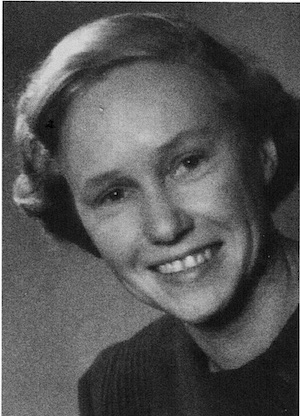
\includegraphics[width=.9\textwidth]{figures/EFJ_young.jpg}
  \caption{Eli Fischer-Jørgensen (1949)}
  \label{fig:ch.hjelmslev.efj-young}
\end{wrapfigure}
Instead, she went to Paris, where she studied phonology with \name{André}{Martinet} (chapter~\ref{ch.martinet} below) and experimental phonetics
with \name{Pierre}{Fouché} and \name{Marguérite}{Durand}, as well as attending lectures
by \name{Émile}{Benveniste} on \ili{Indo-European}. Just before going to Paris, in
July of 1938, she attended the Third International Congress of
Phonetic Sciences in Ghent, where she met {\Jakobson} for the first
time. Following her time in Paris, she was invited to work on
phonetics with \name{Eberhardt}{Zwirner} in Berlin. She was greatly impressed
with {\Zwirner}, but his work was interrupted as a result of political
difficulties, and he was called up for service in the {German} army. She
left Berlin to return to Denmark just two weeks before war broke out.

{\Hammerich} hired {\Eli} as a teaching assistant in \ili{German}, and she was
able to continue her studies in phonetics. In 1943, she was appointed
as a Lecturer in Phonetics, a new post under the chair of linguistics
occupied by {\Hjelmslev}. Opportunities for experimental work in
phonetics were initially quite limited, due to a lack of equipment and
facilities, but gradually through her own efforts and with {\Hjelmslev}'s
support, she developed a laboratory adequate to support her program.

During the {German} occupation of Denmark in World War II, {\Eli} was
engaged in rather dangerous work with the resistance group led by
Prof. \name{Carsten}{Høeg} in assembling files on Nazi collaborators for
prosecution after the war (\citealt[67ff.]{skytte16:eli},
\citealt{efj.ege05:resistance}).

{\Hjelmslev} was already the primary figure in {Danish} linguistics at the
time, and his book \citealt{hjelmslev43:prolegomena}, the main basis
on which his ideas would be known outside Denmark, was the center of
discussion in the Copenhagen circle for many years. Her review of the
book \citep{efj43:rvw.hjelmslev} in the same year served as a landmark
both in the exposition of {\Hjelmslev}'s ideas, introducing these to
students and others in somewhat more readable form, and in their
critical evaluation.

After the war, {\Eli} received a scholarship for a year's study abroad.
On {\Hjelmslev}'s advice, she went to London where she could receive
serious training in phonetics. While there, she attended lectures by
\name{Daniel}{Jones} at University College and also ones by J. R. {\Firth} at the
School of Oriental Studies, as well as doing practical phonetics work
on \ili{English} and \ili{French} with \name{Hélène}{Coustenoble}.

In 1949, she renewed her acquaintance with \name{Roman}{Jakobson}, initiating
a correspondence that continued until his death in 1982. These
letters, collected as \citealt{early.years:efj-rj.letters}, document
an intellectual interaction at times quite sharp but always
cordial. {\Jakobson} was quite interested in discussing the relation
between {\Hjelmslev}'s views and his own theory of distinctive
features. They met in person again when {\Jakobson} visited Copenhagen in
May, 1950, and in 1952 {\Eli} received a Rockefeller Scholarship to visit
the US. She spent five weeks at MIT, where she had a visiting
appointment arranged with {\Jakobson}'s support. He was very eager for
her to spend the rest of the year working on a project with him, but
she found it impossible to stay on. The circumstances are not entirely
clear, but after her departure from Cambridge, her subsequent letters
to him went unanswered until they met again in 1957 at the Eighth
{International Congress of Linguists} in Oslo.

After her stay at MIT, she went to New York to work with the group of
phoneticians at Haskins Laboratories. She was particularly taken with
the possibilities offered for speech synthesis research by the
pattern-playback machine. From there, she went to Oklahoma to study
briefly with \name{Kenneth}{Pike} before returning to Copenhagen. Other
collaborations included a stay in Stockholm in 1954 to work with
\name{Gunnar}{Fant}. {\Eli} always downplayed her \isi{competence} in the domain of
physical \isi{acoustics}, but she was particularly delighted to have been
the official opponent at {\Fant}'s defense of his doctoral thesis
\citep{fant60:acoustic.theory}.

\begin{wrapfigure}[16]{l}{.35\textwidth}
 \includegraphics[width=.9\textwidth]{figures/Eli Fischer-Jørgensen.jpg}
  \caption{Eli Fischer-Jørgensen (1968)}
 \label{fig:ch.hjelmslev.efj}
\end{wrapfigure}
Over the following years, she devoted herself to a rich program of
teaching and research in phonetics. She was appointed to a personal
professorship in phonetics in 1966, associated with the establishment
of her own department, the Institut for Fonetik. The program thrived,
and with it her research and that of her colleagues. In 1968 she was
admitted to the Royal {Danish} Academy of Sciences and Letters, the
first woman to become a domestic member.  In 1979, the Ninth
International Congress of Phonetic Sciences was held in Copenhagen,
largely organized by {\Eli}. In 1981, she reached the mandatory
retirement age and withdrew somewhat (but not toally) from academic
life. She died in February, 2010, soon after her 99th birthday.

It would be hard to argue that \name{Eli}{Fischer-Jørgensen} was a major
innovative figure in the development of phonological theory. As she
says, from her first participation in the discussions of the
\isi{Linguistic Circle of Copenhagen} she ``realized the great difference
between being able to understand a theory and being able to create a
theory'' \citep[63]{fischer-jorgensen81:causerie}. And she contributed
greatly to the field by being able to understand a wide variety of
related but quite different theoretical positions, and to bring that
understanding to bear in confronting those theories with one another's
insights and with the hard facts elicited in the phonetics
laboratory. Familiar at first hand with the work and opinions of
{\Hjelmslev}, {\Jakobson}, {\Martinet}, {\Jones}, {\Firth}, {\Pike} and others, she was
uniquely positioned to provide a balanced view of the comparative
merits and deficiencies of a variety of notions of what ``phonology''
ought to be, as illustrated in her history of the field
\citep{fischer-jorgensen75:trends}.

This was particularly true of her position between {\Hjelmslev} and
{\Jakobson}, two important figures whose views were quite at odds but who
maintained very friendly relations (perhaps dating to the cordial
reception {\Hjelmslev} and other {Danish} linguists offered to {\Jakobson} in
his initial escape from the Germans at the beginning of the war). {\Eli}
was able to bring the arguments of each to bear on the other, and also
to argue against what she saw as the weaknesses in each of their
positions. In both cases, her objections follow from her experience as
a phonetician.

\begin{wrapfigure}[16]{r}{.4\textwidth}
  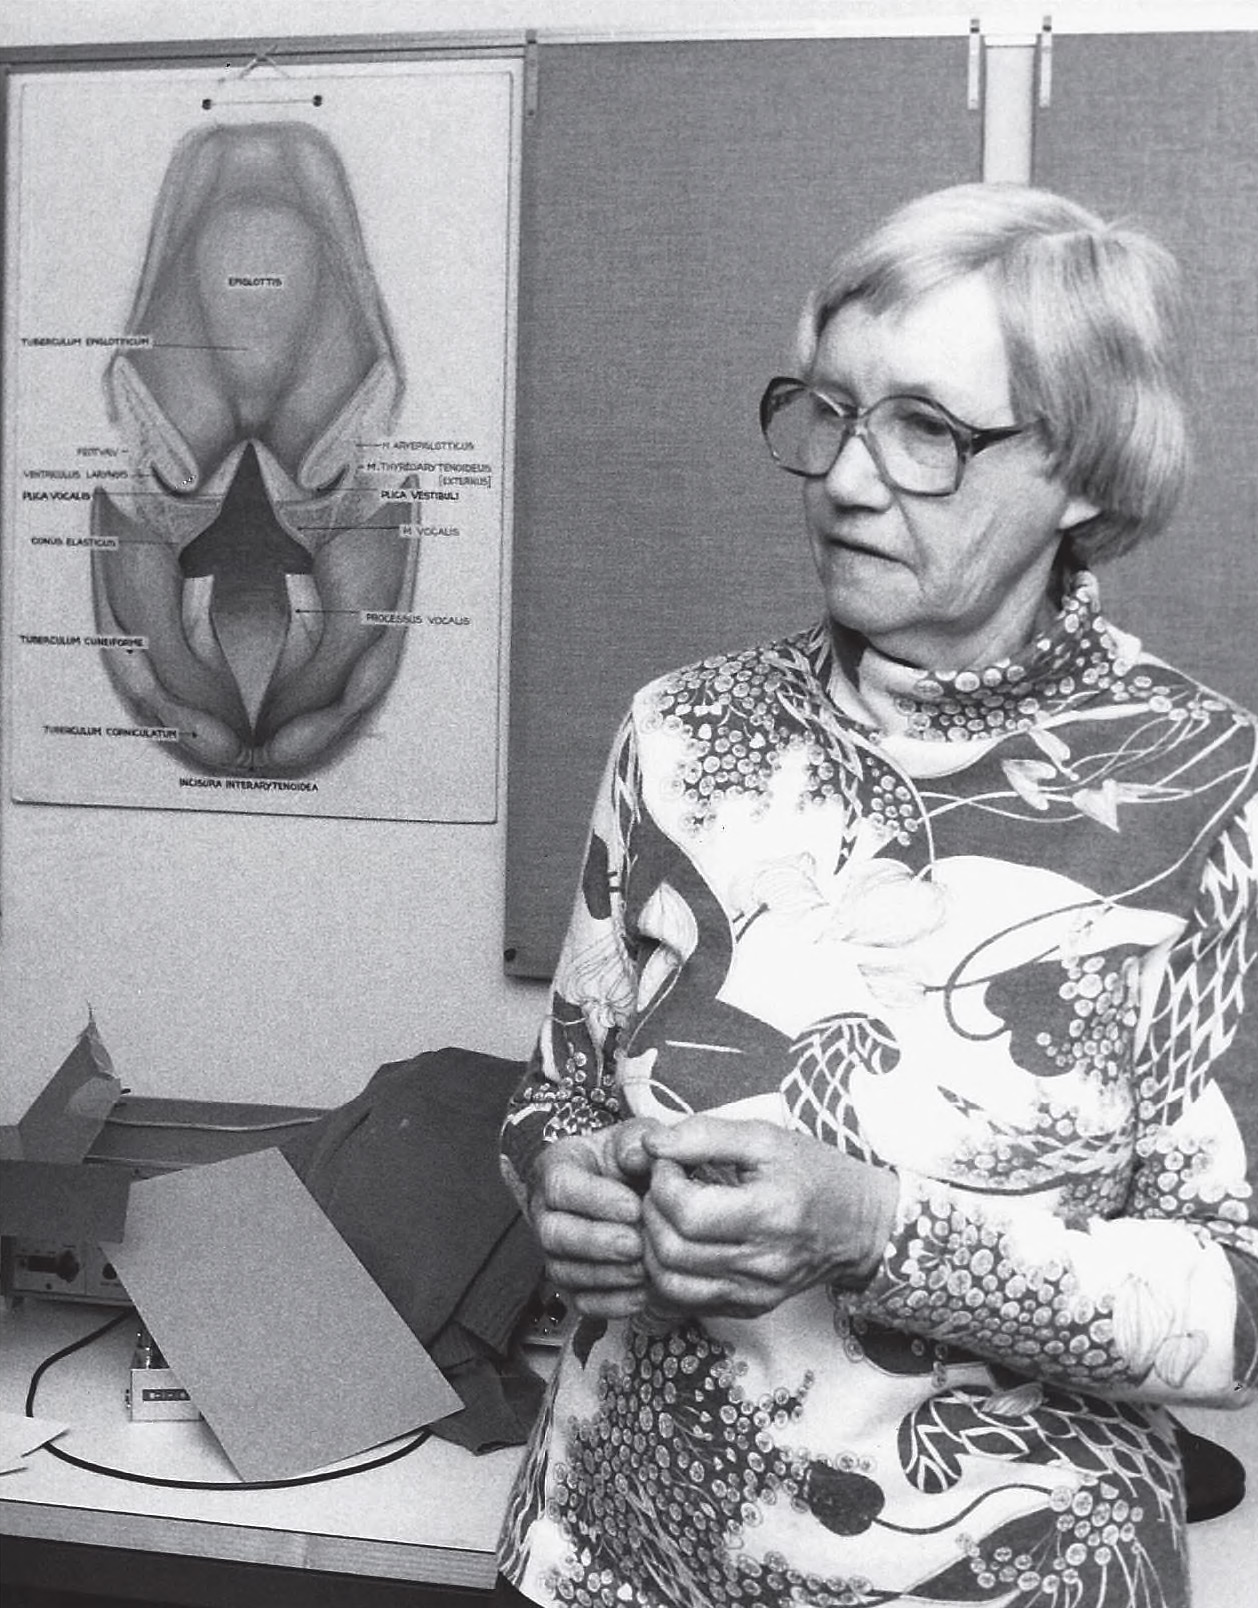
\includegraphics[width=.9\textwidth]{figures/eli_lab.jpg}
  \caption{Eli Fischer-Jørgensen in the Phonetics Lab (1981)}
  \label{fig:ch.hjelmslev.efj_lab}
\end{wrapfigure}
In the case of {\Hjelmslev}'s views, she points out in a series of papers
(including \citealt{efj43:rvw.hjelmslev,efj52:distribution} and
elsewhere) that the Glossematic attempt to analyze linguistic
structure as purely algebraic in character, with no grounding in
phonetic reality on the ``expression'' side, dating back already to
\posscitet{hjelmslev.uldall35:phonematics} London Congress
presentation, could not really be carried out. For one thing, the only
way the realizations of formal elements in different structural
positions could be satisfactorily identified with one another
(e.g. initial {[t]} and post-vocalic {[d]} in \ili{Danish}) must involve at
least an implicit appeal to their phonetic identity. Other specific
problems with important aspects of the theory such as the Commutation
Test \citep{efj56:commutation}, and the overall relation between the
notions of Form and Substance \citep{efj66:form.and.substance} emerged
from her extensive discussions with {\Hjelmslev}, in meetings of the
Copenhagen Linguistic Circle and elsewhere. These differences, along
with areas of agreement between them, are surveyed in
\citealt[chap. 7]{fischer-jorgensen75:trends}.

{\Eli}'s relation to {\Jakobson}'s views was somewhat more nuanced, but
again grounded in her respect for phonetic facts. One point between
them concerned {\Jakobson}'s insistence that phonological features had to
be binary in character, though they agreed to disagree about this.
\begin{quotation}
  I remember once meeting him in America --- it was in the beginning
  of our acquaintance --- and his first words were ``I know you are my
  enemy!'' I was very astonished and asked him how he had got that
  idea, and he answered': ``You do not believe in the binary
  principle''. So I explained that I found the binary principle very
  important, but speaking a language with four degrees of aperture in
  the vowels it was somewhat difficult for me to accept the binary
  principle as an absolute universal. He understood this, and we have
  been friends ever since. \citep[23]{efj97:jakobson}
\end{quotation}

{\Eli}'s respect for {\Jakobson}'s ideas went back to her initial enthusiasm
for the publications of the Prague phonologists, though from the
beginning she had reservations about the extent to which the
phonological perspective was claimed to exclude phonetics, relegating
this to the realm of the natural sciences. It was particularly
\posscitet{jakobson:kindersprache} \textsl{Kindersprache} that
fascinated her, and {\Eli} was generally approving of his efforts to
ground the \isi{distinctive features} in phonetic definitions. Nonetheless,
she had a number of objections to {\Jakobson}'s specific program in this
regard, summarized in
\citealt[162ff.]{fischer-jorgensen75:trends}. Over the years, as
documented in the letters collected by
\citet{early.years:efj-rj.letters}, she showed no reluctance to
challenge {\Jakobson}'s position from the secure basis of her work as a
phonetician.

It seems reasonable to suggest that just as {\Eli}'s view of phonology
was strongly shaped by her training and research in phonetics, so also
the phonetic topics on which she worked extensively (e.g. \ili{Danish}
\emph{stød}, \citealt{efj87:stod}; the properties distinguishing
``voiced'' and ``voiceless'' \isi{stops}, \citealt{efj68:stops} and
elsewhere, etc.) were informed by insights from phonological
analysis. This productive interplay between a variety of approaches to
phonology and the hard data obtained in the phonetics lab
characterized her research program and that of her institute, and was
continued in the way linguistics in Denmark maintained its
significance, through {\Eli}'s students and colleagues such as Jørgen
{\Rischel}, \name{Nina}{Grønnum}, \name{Hans}{Basbøll} and others.

%%% Local Variables: 
%%% mode: latex
%%% TeX-master: "/Users/sra/Dropbox/Docs/Books/P20C_2/LSP/main.tex"
%%% End: 
